\documentclass{article}
\usepackage{xcolor}
\newcommand{\myhighlight}[1]{\textcolor{blue}{#1}}

% The draft follows the supplied NeurIPS-style template when the local style
% file exists, and falls back to a standard preprint layout in this workspace.
\IfFileExists{neurips_2026.sty}{%
  \usepackage{neurips_2026}
}{%
  \usepackage[margin=1in]{geometry}
  \usepackage[numbers,sort&compress]{natbib}
  
}

\usepackage[utf8]{inputenc}
\usepackage[T1]{fontenc}
\usepackage{hyperref}
\usepackage{url}
\usepackage{booktabs}
\usepackage{amsfonts}
\usepackage{amsmath}
\usepackage{nicefrac}
\usepackage{microtype}
\usepackage{xcolor}
\usepackage{enumitem}
\usepackage{tabularx}
\usepackage{array}
\usepackage{graphicx}
\usepackage{tikz}
\usetikzlibrary{arrows.meta, positioning}

\usepackage{mathtools}
\usepackage{amsthm}
\theoremstyle{plain}
% \newtheorem{findings}{Findings}
\newtheorem{desideratum}{Desideratum}
\renewcommand{\thedesideratum}{\Roman{desideratum}}



\hypersetup{
  colorlinks=true,
  linkcolor=blue,
  citecolor=blue,
  urlcolor=blue
}

% \title{A Fault-Tolerant Hierarchical Multi-Agent Protocol for Public-Good Task Production}



\title{\textit{Shared Your Tokens!}  A Protocol for Leveraging Local Tokens  for  Distributed ``Intelligent'' Tasks}
% \title{Shared Token Economics:  A Protocol for Leveraging Local Tokens  for  Distributed ``Intelligent'' Tasks}
 % Verifiable and Scalable
\author{Anonymous Author(s)}

\begin{document}

\maketitle

\begin{abstract}
Large-scale public-good tasks, such as scientific computation, low-resource language documentation, and multi-source data annotation, increasingly require not only generation but also decomposition, verification, revision, and accountable integration. Modern AI systems suggest that useful outputs can often be obtained by spending sufficient tokens; however, the required token, compute, and human-execution resources may exceed the capacity of any single user or organization. Meanwhile, many personal devices, local GPUs, cloud credits, tool-execution environments, and human annotators remain under-utilized.

This paper proposes TokenShare, a protocol for aggregating idle tokens and heterogeneous execution capacity into useful, verifiable work. TokenShare represents a large task as a recursively decomposable task tree or DAG, assigns atomic units to distributed clients, supports local and server-side verification, reassigns failed tasks, recursively merges accepted outputs, and records contributions through a ledger. Unlike proof-of-work systems that coordinate untrusted participants around artificial computation, TokenShare focuses on useful computation with real public-good value. We outline the protocol design, fault-tolerance mechanisms, incentive settlement, and evaluation plan, aiming to measure not only final output quality but also reliability, provenance, recoverability, cost, and verifiability.
\end{abstract}

\section{Introduction}

The infinite monkey theorem offers a useful metaphor for modern AI computation: with enough attempts, even highly complex outputs can in principle be produced. In today’s AI systems, these “attempts” are largely mediated by tokens. For many tasks, better outputs can be achieved by spending more tokens on planning, decomposition, generation, tool use, verification, and revision. In this sense, tokens have become a basic unit of intelligent work.

However, meaningful tasks often require far more than a single prompt-response interaction. Scientific computing, public-health analysis, low-resource language documentation, benchmark construction, and large-scale annotation all require decomposed execution, quality control, expert review, and accountable integration. As task scale increases, the token and compute budget required to complete such work may exceed the capacity of any individual, laboratory, or organization.

At the same time, a large amount of useful capacity remains idle. Personal devices, local GPUs, laboratory servers, browser-based tool environments, cloud credits, human annotators, and user-owned AI agents are often under-utilized. Although each contributor may only provide a small amount of tokens, computation, or time, their aggregated capacity can be substantial.

This motivates the central question of this paper: Can we design a protocol that enables a community to collectively complete useful computational tasks by sharing tokenized resources, while preserving correctness, accountability, and fault tolerance?

We propose TokenShare, a scalable, verifiable, fault-tolerant, and automated protocol for shared token economics. TokenShare represents a large task as a hierarchical task tree or task DAG. A root task is recursively decomposed into subtasks according to the number of available clients, their capability profiles, estimated task complexity, and verification cost. Each atomic task unit is assigned to one or more clients, locally validated before submission, verified again by master or verifier nodes, and recursively merged into higher-level outputs. Through this process, idle tokens and execution capacity are converted into auditable, mergeable, and useful work.

TokenShare is inspired by decentralized systems such as Bitcoin and smart contracts. These systems show that mutually untrusted participants can be coordinated through shared ledgers, commitments, and incentive-compatible rules. Yet Bitcoin’s proof-of-work computation is intentionally artificial: it secures the network but does not directly produce scientific, educational, or public-interest outputs. TokenShare instead asks how distributed tokens, computation, and human/program execution capacity can be organized to complete useful and socially meaningful tasks.

This shift from meaningless computation to useful computation introduces new challenges. Useful tasks require decomposition, capability-aware routing, heterogeneous execution, local and global verification, fault recovery, provenance tracking, and incentive settlement. Contributors may be slow, unreliable, malicious, offline, or equipped with different models and tools. Therefore, the protocol must not only pool resources, but also preserve correctness, recover from failure, and make the final output auditable.

This paper makes three main \textbf{contributions}:

\begin{itemize}
\item We formulate shared token economics as a protocol problem for useful distributed intelligent tasks.
 \item We design TokenShare, a recursive protocol that supports task decomposition, client-side validation, server-side verification, fault recovery, result merging, and token settlement.
\item  We propose an evaluation framework that measures output quality, reliability, verification cost, provenance, recovery, and efficiency rather than only final-answer correctness.
\end{itemize}






\section{Motivation Towards Shared Token Economics}


\subsection{Background}

\textbf{Tokens as the Intelligent Units}~
The infinite monkey theorem offers a useful metaphor for the current moment of AI computation: given a typewriter and infinite time, a monkey would eventually type Shakespeare. The theorem is not practically useful as a method of literary production, but it highlights a basic principle: sufficiently many attempts can, in principle, produce highly complex outputs. Modern AI systems exhibit a similar phenomenon. For many tasks, desirable outputs can often be obtained if enough tokens are spent on generation, decomposition, tool use, verification, revision, and retry. In this sense, tokens have become a basic computational resource for producing useful intellectual work.

\textbf{The Price of Token Economics}~
However, this token-based view also exposes a scaling bottleneck. As tasks become larger, more uncertain, or more socially meaningful, the number of required tokens may exceed the budget of any individual user, laboratory, or organization. Large-scale scientific computing, public-health analysis, low-resource language documentation, benchmark construction, and multi-source data annotation all require not only raw generation, but also planning, decomposition, execution, verification, expert review, and accountable integration. These requirements make the task expensive in terms of tokens, compute, human attention, and tool-execution capacity.


\subsection{Motivations}

At the same time, a large amount of useful capacity remains idle. Personal devices, local GPUs, laboratory servers, cloud credits, browser-based tool environments, human annotators, and user-owned AI agents are often under-utilized. Individually, each contributor may only provide a small amount of tokens, computation, or execution time. Collectively, however, these idle resources may form a substantial pool of distributed capacity.

A natural question is therefore: \emph{Can we design a protocol that allows a community to collectively complete useful computational tasks by sharing tokenized incentives, while ensuring correctness, accountability, and fault tolerance?}


TokenShare addresses this question by proposing a scalable, verifiable, fault-tolerant, and automated protocol for distributed token sharing. The key idea is to represent a large task as a recursively decomposable task tree or task graph. A root task is divided into subtasks; each subtask can be further decomposed according to the number of available clients, their capability profiles, the estimated task complexity, and the cost of verification. Each atomic task unit is assigned to one or more clients, locally validated before submission, verified again by the master or verifier nodes, and recursively merged into higher-level outputs. Through this process, idle tokens are not merely donated or consumed; they are converted into auditable, mergeable, and useful work.

Existing decentralized systems provide an important precedent. Bitcoin demonstrates that a large number of mutually untrusted participants can be coordinated through shared ledgers, cryptographic commitments, and incentive-compatible rules. Smart contracts further show that task states, deposits, rewards, and disputes can be managed by transparent and programmable mechanisms. Yet Bitcoin's proof-of-work computation is intentionally artificial: its computational puzzle secures the network but does not directly produce scientific, educational, or public-interest outputs. TokenShare focuses on a different and more practical problem: how to organize distributed tokens, computational capacity, and human or program execution capacity to complete useful, verifiable, and socially meaningful tasks.

This shift from meaningless computation to useful computation introduces new challenges. Useful tasks are rarely solved by repeated hashing alone. They require task decomposition, capability-aware routing, heterogeneous execution, local and global verification, fault recovery, provenance tracking, and incentive settlement. Contributors may be slow, unreliable, malicious, offline, or equipped with different models and tools. Therefore, the protocol must not only pool resources, but also preserve correctness, recover from failure, and make the final output auditable. TokenShare is designed as a protocol layer for this setting: it recursively decomposes large tasks, allocates atomic work units, verifies submissions, reassigns failed tasks, merges accepted results, and records contributions through a ledger.




% %  shashpear:  it solves anything with enougth tokens.

% broader sense of tokens: tool-generated tokens; 

% % Large-scale tasks need more tokens? rieman conjecture.  it is afforadablke to a single indivisual. 


% % numbers ?



% Large-scale scientific and social-good computing tasks often require substantial computational resources. Examples include protein folding simulation, climate modeling, public-health data analysis, large-scale literature mining, multilingual data annotation, and benchmark construction for artificial intelligence systems. Although these tasks are socially meaningful, they are often difficult to execute at scale because the required computing power, human labor, and verification effort are distributed across many individuals and institutions. At the same time, a large amount of under-utilized computing capacity exists on personal devices, laboratory servers, edge devices, and institutional clusters.



% Existing decentralized systems provide important inspiration. Bitcoin demonstrates that a large number of untrusted participants can coordinate around a shared ledger through cryptographic commitments and incentive-compatible mechanisms. Smart contracts further show that programmable rules can autonomously manage task assignment, reward distribution, and dispute resolution. However, most existing blockchain-based protocols either focus on financial transactions or rely on computational puzzles that do not directly contribute to socially useful work. In contrast, scientific and public-interest computing requires a protocol in which useful tasks can be decomposed, assigned, verified, merged, and rewarded in a reliable and scalable manner.

% This paper proposes a token-sharing protocol for useful distributed computation. The central idea is to represent a large task as a recursively decomposable task tree. A master task can be divided into multiple subtasks; each subtask can further be divided into smaller subtasks depending on the number of available clients and the complexity of the computation. In this way, a task can be dynamically expanded from $N$ subtasks to $N^2$ or even more fine-grained units. This recursive decomposition allows the system to adapt to the current number of participating clients and their available computational capacity.



% The motivation of this work is therefore threefold. First, we aim to transform idle or fragmented computational resources into a coordinated network for socially meaningful tasks. Second, we aim to design a recursive and adaptive task-decomposition protocol that can scale with the number of available clients. Third, we aim to build a verifiable and fault-tolerant incentive mechanism that borrows from blockchain and smart-contract systems, while focusing on useful computation rather than artificial proof-of-work puzzles.

\section{The Design Philosophy}
\subsection{Problem Formulation}

We consider a large computational task $T$ submitted by a task owner. The task may be scientific, educational, public-interest-oriented, or otherwise useful. The goal is to complete $T$ by distributing its computation among a set of clients
\[
\mathcal{C} = \{c_1, c_2, \ldots, c_m\},
\]
where each client has limited and potentially heterogeneous computational capacity.

The task $T$ can be decomposed into a set of subtasks:
\[
T \rightarrow \{T_1, T_2, \ldots, T_N\}.
\]
Each subtask $T_i$ may be further decomposed recursively:
\[
T_i \rightarrow \{T_{i,1}, T_{i,2}, \ldots, T_{i,K_i}\}.
\]
This produces a task tree or task DAG, depending on whether subtasks are independent or share intermediate dependencies. The decomposition depth and branching factor are determined dynamically by the current number of available clients, the estimated complexity of the task, and the verification cost.

Each atomic task unit $u$ is associated with four components:
\[
u = (x_u, f_u, v_u, r_u),
\]
where $x_u$ is the input, $f_u$ is the required computation, $v_u$ is the verification function, and $r_u$ is the reward assigned to the task unit. A client assigned to $u$ computes
\[
y_u = f_u(x_u),
\]
runs local verification
\[
v_u(x_u, y_u) = 1,
\]
and submits the result together with metadata, logs, and optional cryptographic commitments.



\subsection{Desiderata of TokenShare Protocol}


\begin{desideratum}
\textbf{Decomposability:}~ A TokenShare task should be expressible as a structured task tree or directed acyclic graph whose executable units have clear inputs, outputs, dependencies, and merge relations.
\end{desideratum}

A TokenShare task must be decomposable into smaller executable units. Instead of treating a large task as a single indivisible request, the protocol represents it as a structured task tree or directed acyclic graph. Each node corresponds to a task unit, and each edge represents a decomposition, dependency, review, or aggregation relationship. This design allows a complex task to be divided across multiple agents, workers, or token contributors while preserving the logical structure of the original task.

Decomposability is essential because the protocol assumes that no single contributor may have enough tokens, compute, time, or expertise to complete the entire task. Each decomposed unit should therefore have a clear input, expected output, execution boundary, and dependency relation. For example, a factorization task can be decomposed into divisor-range search units, an annotation task can be decomposed into data batches, and a Lean theorem-proving task can be decomposed into intermediate lemmas or subgoals.


\begin{desideratum}
\textbf{Local Verifiability:}~ Each executable subtask should include an explicit verifier that can check whether its submitted output is valid before that output is accepted, merged, or rewarded.
\end{desideratum}

Each executable subtask must be verifiable before its output is accepted, merged, or rewarded. Local verifiability means that a subtask result should not be trusted simply because a worker submits it. Instead, the protocol must define explicit verification rules for checking whether the output is valid, complete, and consistent with the task specification.

Verification can take different forms depending on the task type. For deterministic computational tasks, the verifier may directly check mathematical correctness, such as whether a candidate factor divides the original number. For data annotation tasks, the verifier may check label schema validity, inter-annotator agreement, or reviewer approval. For formal reasoning tasks, such as Lean theorem proving, the verifier can be an external formal system that checks whether a proof compiles successfully. This requirement prevents invalid intermediate outputs from contaminating the final result.


\begin{desideratum}
\textbf{Extendability:}~ The protocol should provide a reusable coordination skeleton while allowing each task family to plug in task-specific schemas, verifiers, merge rules, cost models, and contributor requirements.
\end{desideratum}

The protocol should be extendable across different task families while allowing each task type to define its own task-specific interface. TokenShare is not designed for only one fixed workflow. Instead, it provides a general protocol skeleton that can be reused across computational tasks, annotation tasks, formal reasoning tasks, and other distributed intelligent tasks.

Extendability requires that each task domain can plug in its own decomposition strategy, input schema, output schema, verification rule, merge rule, cost model, and contributor requirements. For instance, the merge rule for factorization is mathematical recomposition, the merge rule for annotation may be majority voting or reviewer arbitration, and the merge rule for Lean may be the composition of verified lemmas into a final theorem. In this sense, the protocol is general at the coordination level but task-specific at the execution and verification level.


\begin{desideratum}
\textbf{Scalability:}~ As more tokens, agents, workers, or computational resources become available, the protocol should convert that additional capacity into faster completion, higher quality, broader verification, or stronger fault tolerance.
\end{desideratum}

The protocol should become more useful as more tokens, agents, workers, or computational resources become available. When additional contributors join the system, the protocol should be able to decompose tasks into finer-grained units, assign them in parallel, and improve either completion speed, output quality, verification coverage, or fault tolerance.

However, scalability does not simply mean adding more agents. A poorly structured multi-agent system may create redundant work, inconsistent outputs, or excessive coordination overhead. Therefore, TokenShare must scale through explicit task graphs, dependency management, routing policies, verification rules, and merge mechanisms. The goal is not merely to use more agents, but to make additional contributors produce useful, verifiable, and mergeable work.


\begin{desideratum}
\textbf{Autonomy:}~ The protocol should advance tasks through assignment, execution, validation, verification, merging, timeout recovery, reassignment, and settlement according to predefined rules with minimal continuous manual coordination.
\end{desideratum}

The protocol should support autonomous task progression with minimal continuous manual coordination. Once a task enters the protocol, its units should move through assignment, execution, validation, submission, verification, merging, timeout handling, reassignment, and settlement according to predefined protocol rules. This allows the system to operate even when contributors are heterogeneous, unreliable, temporarily offline, or only partially observable.

Autonomy does not mean removing human judgment entirely. Human experts may still be needed for high-risk disputes, ambiguous outputs, culturally sensitive content, or domain-specific validation. However, routine transitions should be handled by the protocol itself. Expired tasks should be requeued, invalid outputs should be rejected, verified outputs should be accepted, and rewards should be settled according to explicit rules. This makes TokenShare closer to a protocol-governed task production system rather than an ad hoc multi-agent conversation.



\section{The TokenShare Protocol}

We propose the \textbf{TokenShare Protocol}, a recursive token-incentivized protocol for useful distributed computation. The protocol contains five major stages: task registration, recursive decomposition, client-side computation and validation, server-side verification and merging, and token settlement.

\subsection{Overall Picture}


\textbf{System Roles}~
The protocol involves the following roles:

\begin{itemize}
    \item \textbf{Task Owner}: The entity that submits a large task and provides the initial reward budget.
    \item \textbf{Master Node}: The coordinating node responsible for maintaining the task tree, assigning subtasks, and merging verified results.
    \item \textbf{Client Nodes}: Participants who perform computation on assigned task units.
    \item \textbf{Verifier Nodes}: Optional nodes that independently verify submitted results, especially for non-trivial or high-value subtasks.
    \item \textbf{Smart Contract}: A programmable ledger component that records task states, commitments, submissions, deposits, and rewards.
\end{itemize}

In a fully decentralized implementation, the master node can be replaced by a smart-contract-controlled coordination layer. In a semi-decentralized implementation, the master node performs orchestration while the smart contract provides transparency and reward enforcement.


\begin{figure}[htbp]
\centering
\resizebox{\linewidth}{!}{
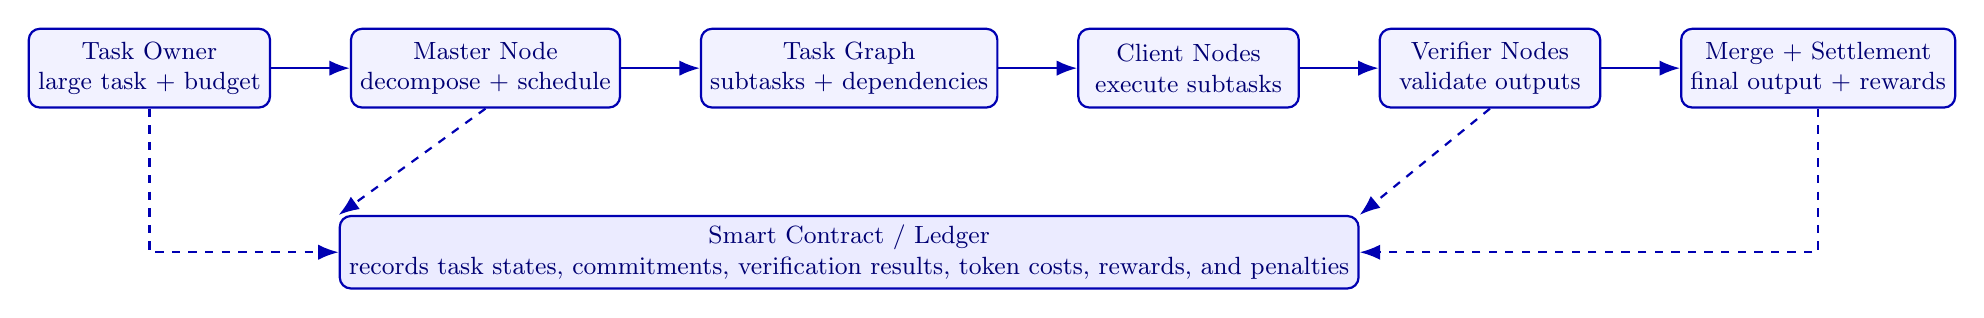
\begin{tikzpicture}[
    node distance=1.0cm and 1.0cm,
    bluebox/.style={
        rectangle,
        rounded corners,
        draw=blue!70!black,
        fill=blue!5,
        thick,
        align=center,
        minimum width=2.8cm,
        minimum height=1.0cm,
        font=\small,
        text=blue!45!black
    },
    ledgerbox/.style={
        rectangle,
        rounded corners,
        draw=blue!70!black,
        fill=blue!8,
        thick,
        align=center,
        minimum width=7.0cm,
        minimum height=0.9cm,
        font=\small,
        text=blue!45!black
    },
    arrow/.style={
        -{Latex[length=2.6mm]},
        thick,
        draw=blue!70!black
    },
    dashedarrow/.style={
        -{Latex[length=2.6mm]},
        thick,
        dashed,
        draw=blue!70!black
    }
]

% Main pipeline
\node[bluebox] (owner) {Task Owner\\large task + budget};

\node[bluebox, right=of owner] (master) {Master Node\\decompose + schedule};

\node[bluebox, right=of master] (graph) {Task Graph\\subtasks + dependencies};

\node[bluebox, right=of graph] (clients) {Client Nodes\\execute subtasks};

\node[bluebox, right=of clients] (verifier) {Verifier Nodes\\validate outputs};

\node[bluebox, right=of verifier] (merge) {Merge + Settlement\\final output + rewards};

% Ledger layer
\node[ledgerbox, below=1.35cm of graph] (ledger) {Smart Contract / Ledger\\records task states, commitments, verification results, token costs, rewards, and penalties};

% Main arrows
\draw[arrow] (owner) -- (master);
\draw[arrow] (master) -- (graph);
\draw[arrow] (graph) -- (clients);
\draw[arrow] (clients) -- (verifier);
\draw[arrow] (verifier) -- (merge);

% Ledger arrows
\draw[dashedarrow] (owner.south) |- (ledger.west);
\draw[dashedarrow] (master.south) -- (ledger.north west);
\draw[dashedarrow] (verifier.south) -- (ledger.north east);
\draw[dashedarrow] (merge.south) |- (ledger.east);

\end{tikzpicture}
}
\caption{Overall architecture of the TokenShare protocol. A task owner submits a large task and an initial budget. The master node decomposes the task into a hierarchical task graph, assigns subtasks to client nodes, verifies submitted outputs through verifier nodes, merges accepted results, and records task states, contribution, cost, and settlement information through the ledger.}
\label{fig:tokenshare-overall}
\end{figure}


\subsection{Task Registration, Decomposition, Assignment, and Commitment}

\subsubsection{Task Registration}

A task owner first registers a large task $T$ by submitting a task specification:
\[
\mathcal{S}_T = (D_T, I_T, F_T, V_T, B_T, \tau_T),
\]
where $D_T$ is the task description, $I_T$ is the input data or input reference, $F_T$ is the computation specification, $V_T$ is the verification rule, $B_T$ is the total token budget, and $\tau_T$ is the deadline. This specification defines not only what the task asks the system to produce, but also how the output should be verified, how much resource is available, and when the task should be completed.

After registration, the protocol creates a task record with status \texttt{Registered}. The master node then analyzes whether the task can be executed directly or should be decomposed into smaller executable units. In this sense, task registration is the entry point of the protocol: it turns an informal user request into a structured object that can be decomposed, assigned, verified, merged, and settled.

\subsubsection{Recursive Task Decomposition}

The master node decomposes the root task according to a decomposition function:
\[
\mathcal{D}(T, m, \rho) \rightarrow \{T_1, T_2, \ldots, T_N\},
\]
where $m$ is the number of currently available clients and $\rho$ represents resource and reliability estimates, such as average compute capacity, expected failure rate, model quality, network availability, and verification cost. The number of subtasks is not fixed. Instead, it is determined adaptively according to the available resource pool.

A simple adaptive rule is:
\[
N = \alpha m,
\]
where $\alpha$ is an oversubscription factor used to handle client heterogeneity and potential failures. If $\alpha > 1$, the system creates more task units than active clients, allowing fast or reliable clients to continue accepting additional work while slower clients are still executing their assigned tasks.

Each subtask can be further decomposed if it remains too large, too costly, or too difficult to verify:
\[
T_i \xrightarrow{\mathcal{D}} \{T_{i,1}, T_{i,2}, \ldots, T_{i,K_i}\}.
\]
This process continues until each leaf task satisfies an atomicity condition:
\[
\text{cost}(T_u) \leq \theta_c
\quad \text{and} \quad
\text{verify}(T_u) \leq \theta_v,
\]
where $\theta_c$ is the maximum acceptable computation cost for a client and $\theta_v$ is the maximum acceptable verification cost.

The resulting task structure is represented as a task graph:
\[
\mathcal{T} = (V,E),
\]
where each vertex represents a task unit and each edge represents a decomposition, dependency, review, or aggregation relation. If subtasks are purely hierarchical, the structure is a tree. If subtasks share intermediate dependencies, the structure becomes a directed acyclic graph.

\subsubsection{Task Assignment and Commitment}

After decomposition, the router assigns leaf task units to clients according to their capability, availability, cost, reliability, and the verification requirement of the task. This assignment is not merely an informal scheduling decision. Before a client starts computation, it accepts a task unit $u$ and submits a cryptographic commitment:
\[
\mathrm{com}_u = H(c_i, u, t, s_i),
\]
where $H$ is a cryptographic hash function, $c_i$ is the client identity, $u$ is the assigned task unit, $t$ is the timestamp, and $s_i$ is a client-side nonce. This commitment binds the client to the assigned unit before execution and prevents the client from changing its claimed assignment after observing other clients' submissions.

The ledger records the assignment state as:
\[
(c_i, u, \mathrm{com}_u, \texttt{Assigned}).
\]
Optionally, the client may deposit a small stake. If the client fails to submit a valid result before the deadline, the task unit can be returned to the task pool and reassigned to another client. The client may also lose part of its stake or reputation score. Therefore, assignment and commitment connect task ownership, execution responsibility, timeout handling, and later settlement into one auditable protocol step.

\subsection{Execution, Verification, Recursive Merge, and Settlement}

\subsubsection{Client-Side Execution and Local Validation}

After receiving an assigned task unit $u$, the client performs the required computation:
\[
y_u = f_u(x_u),
\]
where $x_u$ is the input of the task unit, $f_u$ is the required computation or operation, and $y_u$ is the produced output.

Before uploading the result, the client performs local validation:
\[
v_u(x_u, y_u) = 1.
\]
The validation function may include format checking, boundary checking, consistency checking, deterministic recomputation on small samples, numerical tolerance checking, or other task-specific validity checks. The purpose of local validation is to prevent obviously invalid or incomplete results from entering the global verification pipeline.

The client then submits a result package:
\[
\mathcal{R}_u = (u, y_u, q_u, \pi_u, \mathrm{log}_u),
\]
where $q_u$ is an optional quality score estimated by the client, $\pi_u$ is an optional proof or certificate, and $\mathrm{log}_u$ contains execution metadata such as runtime, software version, hardware information, random seeds, and tool configuration. This metadata is important because TokenShare is designed for heterogeneous contributors whose machines, models, tools, and execution environments may differ.

\subsubsection{Server-Side Verification}

Once a result is submitted, the master node or verifier nodes perform server-side verification. If the task has a deterministic checker, the verifier directly evaluates:
\[
V_u(x_u, y_u) = 1.
\]
This mode is suitable for tasks such as factorization, SAT solving, theorem proving, data transformation, or other computations whose outputs are easy to check.

For tasks that are difficult to verify directly, the protocol may use redundant verification. The same task unit can be assigned to multiple clients:
\[
u \rightarrow \{c_a, c_b, c_c\}.
\]
The result is accepted only if independent submissions satisfy a quorum rule:
\[
\mathrm{Accept}(y_u)=
\begin{cases}
1, & \text{if } \#\{c_i : y_u^{(i)} = y_u\} \geq q,\\
0, & \text{otherwise}.
\end{cases}
\]
For numerical tasks, exact equality can be replaced with a tolerance condition:
\[
\|y_u^{(i)} - y_u^{(j)}\| \leq \epsilon.
\]

The protocol may also support randomized auditing, reviewer judgment, expert escalation, or cryptographic proofs. Randomized auditing allows the system to inspect a subset of completed tasks more deeply. Expert escalation is useful for high-risk or domain-sensitive tasks. Cryptographic proofs, such as Merkle proofs or zero-knowledge proofs, may be used when verification cost is high but formal proof of correctness is possible.

\subsubsection{Recursive Result Merging}

After leaf-level task outputs are verified, accepted results are merged recursively. For a parent task $T_i$ with verified child outputs
\[
\{y_{i,1}, y_{i,2}, \ldots, y_{i,K_i}\},
\]
the master computes:
\[
y_i = M_i(y_{i,1}, y_{i,2}, \ldots, y_{i,K_i}),
\]
where $M_i$ is the merge function associated with the parent task.

The merged result must also pass validation:
\[
V_i(x_i, y_i) = 1.
\]
If the merge fails, the protocol identifies suspicious child tasks, reopens the relevant verification path, and may reassign failed or disputed task units to other clients. In this way, verification is not limited to leaf-level computation. It is applied recursively throughout the task graph, ensuring that accepted subtasks can be recombined into a coherent and valid final output.

\subsubsection{Token Settlement}

Once a task unit or merged output is verified and accepted, the ledger updates the task state, contribution record, and token settlement. A successful client receives a reward:
\[
R(c_i,u)=r_u \cdot \gamma_i \cdot \lambda_u,
\]
where $r_u$ is the base reward for task unit $u$, $\gamma_i$ is the reputation multiplier of client $c_i$, and $\lambda_u$ is the difficulty multiplier.

If the client submits an invalid result, misses the deadline, abandons the task, or is detected as malicious, the protocol may apply a penalty:
\[
P(c_i,u)=s_i \cdot \delta,
\]
where $s_i$ is the client stake and $\delta$ is the penalty ratio. The ledger then updates the client balance:
\[
B(c_i) \leftarrow B(c_i) + R(c_i,u) - P(c_i,u).
\]

Through this process, TokenShare connects execution, verification, recursive merging, and settlement into a single auditable workflow. A submitted result is not accepted merely because it exists. It must pass local validation, server-side verification, merge-level validation, and ledgered settlement before becoming part of the final output.




\section{A Robust Fault-Tolerance Mechanism}

Fault tolerance is central to TokenShare because failures are not exceptional in a heterogeneous token-sharing network. Clients may crash, become slow, go offline, submit low-quality outputs, hallucinate, collude, or act maliciously. Verifiers and coordinators may also fail. Inspired by failure detectors, MapReduce-style re-execution, replicated storage, consensus protocols, Byzantine fault tolerance, and crowdsourcing quality aggregation , TokenShare treats fault tolerance as a closed-loop protocol rather than a single timeout rule.

\subsection{Failure Model}

TokenShare distinguishes seven failure classes:
\begin{itemize}
\item \textbf{Crash failures}: a client, verifier, or coordinator stops responding.
\item \textbf{Omission failures}: a node remains online but misses messages, uploads incomplete artifacts, or fails to checkpoint.
\item \textbf{Stragglers}: a node makes progress but is too slow relative to the task deadline.
\item \textbf{Semantic failures}: an output is syntactically valid but factually wrong, unverifiable, low quality, or unmergeable.
\item \textbf{Byzantine failures}: a participant fabricates logs, submits adversarial outputs, copies another worker's output, or colludes with verifiers.
\item \textbf{Verifier failures}: a verifier rejects valid work, accepts invalid work, or uses an inconsistent environment.
\item \textbf{Control-plane failures}: task state, leases, reward records, or merge dependencies become unavailable or inconsistent.
\end{itemize}

This model is stricter than ordinary distributed computation because TokenShare must tolerate both machine failures and intelligent-work failures.

\subsection{Task State and Idempotent Work Units}

Each task unit is represented as
\[
u=(x_u, f_u, v_u, m_u, b_u, \tau_u, \rho_u, e_u),
\]
where $x_u$ is the input, $f_u$ is the required computation, $v_u$ is the verifier, $m_u$ is the merge rule, $b_u$ is the budget, $\tau_u$ is the lease deadline, $\rho_u$ is a risk score, and $e_u$ is the required execution environment. Each attempt has a unique tuple
\[
a=(u,\ell,c,h_x,h_e,t),
\]
where $\ell$ is the lease id, $c$ is the client id, $h_x$ is the input hash, $h_e$ is the environment hash, and $t$ is the attempt timestamp.

All work units are idempotent: re-running the same unit must not corrupt global state. Outputs are written to temporary, content-addressed artifacts and become visible only after verification. Settlement is also idempotent: a reward event is keyed by $(u,\ell,c)$, so retries cannot create duplicate payment.

\subsection{Lifecycle State Machine}

A task unit moves through the following states:
\[
\textsc{Ready} \rightarrow \textsc{Leased} \rightarrow \textsc{Running}
\rightarrow \textsc{Submitted} \rightarrow \textsc{Verified}
\rightarrow \textsc{Merged} \rightarrow \textsc{Settled}.
\]
Failure transitions include:
\[
\textsc{Leased} \rightarrow \textsc{Expired},\quad
\textsc{Running} \rightarrow \textsc{Straggler},\quad
\textsc{Submitted} \rightarrow \textsc{Rejected},\quad
\textsc{Submitted} \rightarrow \textsc{Disputed}.
\]
Expired, rejected, and disputed units return to the ready pool with their evidence preserved. A failed attempt is never simply deleted; it becomes training signal for routing, reputation, verifier auditing, and later repair.

\subsection{Failure Detection}

Timeout alone is too crude. TokenShare maintains a suspicion score
\[
\sigma(c,u,t)=
w_1 H(c,t)+w_2 P(c,u,t)+w_3 Q(c,u)+w_4 R(c),
\]
where $H$ measures missing heartbeats, $P$ measures abnormal progress, $Q$ measures local validation failures, and $R$ measures historical unreliability for this task type. A client is not immediately punished when $\sigma$ is high; instead, the scheduler first reduces the lease length, starts a shadow attempt, or asks for a checkpoint. Penalties are applied only after the evidence distinguishes honest failure from invalid or malicious behavior.

\subsection{Adaptive Redundant Assignment}

Each task unit receives a redundancy level
\[
k_u=\min(k_{\max},\max(1,\lceil \log(\epsilon_u)/\log(\hat{p}_u)\rceil)),
\]
where $\epsilon_u$ is the tolerated probability that all assigned attempts fail, and $\hat{p}_u$ is the estimated failure probability for the selected client pool. High-risk tasks, subjective tasks, culturally sensitive tasks, high-reward tasks, and tasks with weak verifiers receive larger $k_u$. Low-risk deterministic tasks may start with one worker plus random audit.

Redundant assignment must be diverse. The $k_u$ workers should differ in model family, hardware, geographic region, prior collaboration graph, and reputation profile when possible. This prevents correlated hallucinations, shared tool bugs, and collusive outputs from being mistaken for agreement.

\subsection{Straggler Mitigation and Checkpoint Recovery}

When a task becomes a straggler, TokenShare launches a speculative shadow attempt rather than waiting for the original lease to expire. The first attempt that passes verification becomes the canonical result. If both succeed, the later result may still be used as audit evidence but does not receive full completion reward.

For long tasks, clients must submit checkpoints:
\[
\chi_i=(u,\ell,i,h_{\mathrm{state}},h_{\mathrm{log}},t_i).
\]
A checkpoint is useful only if it can be replayed or validated. If a client disappears, the scheduler resumes from the latest verified checkpoint instead of restarting from scratch. If checkpoint replay fails, the attempt is marked non-reproducible and its reputation impact is stronger than an ordinary timeout.

\subsection{Verification Committees}

TokenShare uses tiered verification.

For deterministic tasks, such as integer factorization or Lean proof checking, one canonical verifier may be sufficient, but high-value outputs are randomly audited by independent verifiers. For semantic tasks, such as annotation or low-resource language artifacts, TokenShare uses a verifier committee. An output is accepted only if
\[
\sum_{j\in V_u} r_j \cdot \mathbf{1}[v_j(y_u)=1] \geq \theta_u,
\]
where $r_j$ is verifier reliability and $\theta_u$ is a task-specific acceptance threshold.

For adversarial or high-stakes tasks, the committee size follows a Byzantine assumption: tolerating $f$ faulty verifiers requires at least $3f+1$ committee members and a quorum of $2f+1$ consistent decisions. This is more expensive, so it is reserved for tasks where an invalid merge would be costly.

\subsection{Semantic Quality Aggregation}

Not all useful work has a deterministic verifier. For annotation, review, language documentation, and open-ended generation, TokenShare estimates latent quality rather than relying on majority vote. It tracks worker ability, item difficulty, and consensus confidence using Dawid--Skene-style aggregation, GLAD-style difficulty modeling, MACE-style trust estimation, or CrowdLab-style model-assisted quality scoring \citep{dawid1979maximum,whitehill2009glad,hovy2013mace,goh2023crowdlab}.

A semantic unit is accepted only when its confidence exceeds a threshold:
\[
\Pr(y_u=\hat{y}_u \mid A_u,W_u,D_u) \geq \gamma_u,
\]
where $A_u$ is the set of submitted answers, $W_u$ is worker reliability, and $D_u$ is estimated task difficulty. Low-confidence items are escalated to expert review rather than silently merged.

\subsection{Reputation, Stake, and Delayed Settlement}

Each client has a vector-valued reputation, not a single score:
\[
R_c=(R_c^{\mathrm{latency}},R_c^{\mathrm{validity}},R_c^{\mathrm{semantic}},R_c^{\mathrm{replay}},R_c^{\mathrm{dispute}}).
\]
This prevents a client that is good at cheap deterministic tasks from being trusted automatically on expert semantic tasks. Reputation is updated only after verification and, for decompositions, after the parent merge succeeds.

Rewards are delayed until the contribution is usable. Direct outputs receive reward after verification. Decomposition proposals receive provisional credit, but final reward is released only if child tasks verify and the parent merge succeeds. Malicious submissions, non-replayable logs, fabricated environments, or verifier collusion trigger stake loss and reputation decay. Honest timeouts reduce scheduling priority but do not receive the same penalty as adversarial behavior.

\subsection{Dispute Resolution}

A task enters \textsc{Disputed} when redundant outputs conflict, verifier decisions disagree, or a parent merge fails. Dispute resolution proceeds in four stages:
\begin{enumerate}
\item \textbf{Replay}: rerun deterministic verification in the canonical environment.
\item \textbf{Independent audit}: assign the task to fresh workers or verifiers with no recent collaboration link to the disputed parties.
\item \textbf{Weighted aggregation}: use reputation- and difficulty-aware aggregation for semantic tasks.
\item \textbf{Expert arbitration}: escalate only the minimal conflicting artifact, not the whole task tree.
\end{enumerate}
The winning output is merged; losing outputs remain in the ledger as negative or ambiguous evidence. This preserves auditability and prevents repeated disputes from being invisible.

\subsection{Control-Plane Fault Tolerance}

The task graph, lease table, verifier decisions, checkpoint hashes, merge records, and settlement events are stored in an append-only event log. The coordinator can be replicated using a crash-fault-tolerant protocol such as Raft \citep{ongaro2014raft}. For adversarial deployments, verifier and settlement committees may use Byzantine replication ideas \citep{castro1999pbft}. Periodic snapshots compact the event log, but snapshots are accepted only if their hash matches the replayed task state.

The control plane therefore satisfies three properties:
\begin{itemize}
\item \textbf{Recoverability}: after coordinator failure, the system reconstructs all task states from the event log.
\item \textbf{No double settlement}: reward events are idempotent and keyed by verified attempts.
\item \textbf{Auditable provenance}: every merged artifact links to its input hash, worker, verifier, lease, environment, logs, and settlement event.
\end{itemize}

\subsection{Fault-Tolerance Summary}

TokenShare does not rely on one mechanism. Its stability comes from layered defense: leases detect disappearance, speculative execution handles stragglers, checkpoints reduce wasted work, adaptive redundancy handles uncertainty, verifier committees handle invalid outputs, semantic aggregation handles noisy judgment, reputation and stake discourage repeated bad behavior, and replicated event logs protect the control plane. The result is a protocol that can degrade gracefully: failures may increase cost or delay, but they should not silently corrupt the final artifact or reward ledger.


% \section{Protocol Lifecycle}

% The complete lifecycle of the protocol is as follows:

% \begin{enumerate}
%     \item The task owner registers a useful computation task and deposits tokens.
%     \item The master node decomposes the task into subtasks according to available clients.
%     \item Subtasks are recursively decomposed until atomic task units are produced.
%     \item Clients accept task units and submit cryptographic commitments.
%     \item Clients compute results and perform local validation.
%     \item Clients upload results, logs, and optional proofs.
%     \item The master node or verifier nodes perform server-side verification.
%     \item Verified leaf results are recursively merged into higher-level results.
%     \item Invalid, missing, or disputed tasks are reassigned.
%     \item Rewards and penalties are settled automatically through the smart contract.
% \end{enumerate}





\section{Proof of Concept Applications}



The two applications instantiate the same protocol skeleton but stress different properties. Large integer factorization is a clean systems benchmark with cheap deterministic verification. Lean formal proof production is a token-consuming intelligent-work benchmark with recursive decomposition and deterministic replay. Figure~\ref{fig:poc_workflow} summarizes the common experiment loop.

{
\begin{figure}[t]
\centering
\resizebox{\linewidth}{!}{%
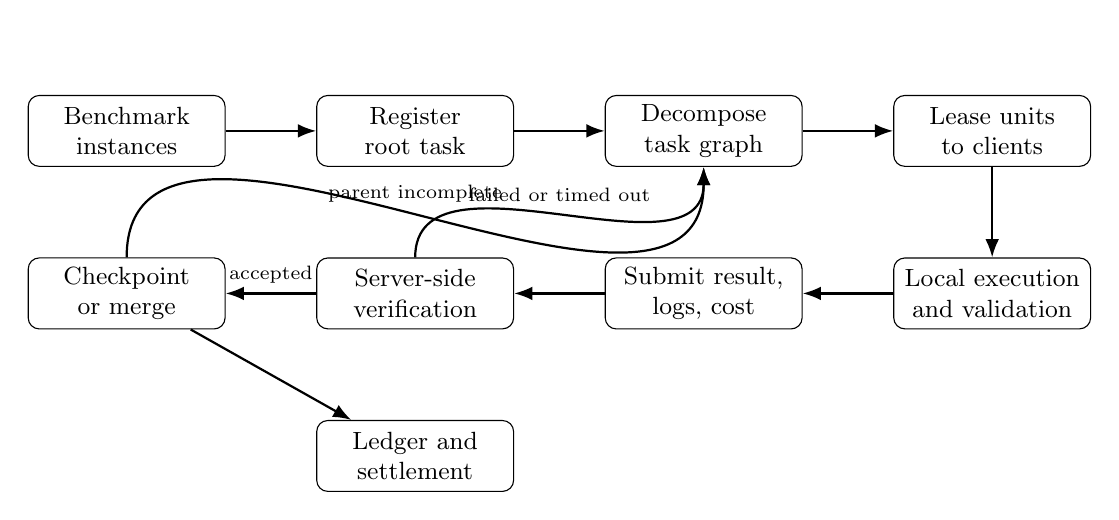
\begin{tikzpicture}[
  node distance=1.15cm,
  box/.style={draw, rounded corners, align=center, minimum width=2.5cm, minimum height=0.9cm, font=\small},
  smallbox/.style={draw, rounded corners, align=center, minimum width=2.2cm, minimum height=0.8cm, font=\small},
  arrow/.style={-Latex, thick}
]
\node[box] (bench) {Benchmark\\instances};
\node[box, right=of bench] (register) {Register\\root task};
\node[box, right=of register] (decompose) {Decompose\\task graph};
\node[box, right=of decompose] (lease) {Lease units\\to clients};
\node[box, below=of lease] (execute) {Local execution\\and validation};
\node[box, left=of execute] (submit) {Submit result,\\logs, cost};
\node[box, left=of submit] (verify) {Server-side\\verification};
\node[box, left=of verify] (merge) {Checkpoint\\or merge};
\node[box, below=of verify] (settle) {Ledger and\\settlement};

\draw[arrow] (bench) -- (register);
\draw[arrow] (register) -- (decompose);
\draw[arrow] (decompose) -- (lease);
\draw[arrow] (lease) -- (execute);
\draw[arrow] (execute) -- (submit);
\draw[arrow] (submit) -- (verify);
\draw[arrow] (verify) -- node[above, font=\scriptsize] {accepted} (merge);
\draw[arrow] (merge) -- (settle);
\draw[arrow] (verify.north) to[out=90,in=270] node[above, font=\scriptsize] {failed or timed out} (decompose.south);
\draw[arrow] (merge.north) to[out=90,in=270] node[above, font=\scriptsize] {parent incomplete} (decompose.south);
\end{tikzpicture}}
\caption{Common proof-of-concept workflow. Each benchmark instance is registered as a root task, expanded into claimable units, executed by heterogeneous clients, verified by task-specific checkers, and either checkpointed, merged, reassigned, or settled.}
\label{fig:poc_workflow}
\end{figure}

\begin{table}[t]
\caption{How the two applications instantiate TokenShare.}
\label{tab:poc_applications}
\centering
\small
\begin{tabularx}{\linewidth}{p{0.18\linewidth}XX}
\toprule
Component & Large integer factorization & Lean formal proof production \\
\midrule
Root task & Factor a composite integer $n$, typically a semiprime $n=pq$. & Prove a theorem statement $s$ under fixed imports and environment $\Omega$. \\
Task unit & Search range $I_j$, algorithmic stage, or intermediate artifact. & Proof state, subgoal, or auxiliary lemma. \\
Decomposition & Partition search ranges or split algorithmic stages such as relation collection and filtering. & Generate subgoals, auxiliary lemmas, or mergeable proof plans. \\
Submission & Factor candidate, negative range certificate, or intermediate relation artifact. & Lean proof patch, decomposition object, error log, and token/tool metadata. \\
Verifier & Check $1<d<n$ and $n\bmod d=0$; replay or audit negative certificates. & Rebuild the Lean project in the canonical environment. \\
Recovery & Requeue expired ranges; reuse verified negative ranges and intermediate artifacts. & Requeue failed proof states; reuse verified subproofs and error logs. \\
Main metrics & Completion time, duplicated ranges, client utilization, recovery time, reward per factorization. & Proof success rate, token cost per theorem, valid decomposition rate, merge success, checkpoint reuse. \\
\bottomrule
\end{tabularx}
\end{table}


\subsection{Application I: Large Integer Factorization}

The first proof-of-concept application is large integer factorization. More precisely, the task owner submits a composite integer $n$, such as a semiprime $n=pq$, and the goal is to recover a non-trivial factorization. This application is useful as an initial benchmark because it is difficult to solve by naive search, naturally parallelizable, and has an extremely cheap deterministic verifier: a submitted factor $d$ is valid if $1<d<n$ and $d \mid n$. Unlike the main TokenShare motivation, this task is not primarily token-driven language generation. Its role is to test the protocol layer under a clean computational workload where decomposition, leases, redundant execution, recovery, verification, and settlement can be measured without subjective judgment.

\paragraph{Task specification.}
The registered task is
\[
\mathcal{S}_{\mathrm{fac}}=(n,\mathcal{A},B,\tau,\kappa),
\]
where $n$ is the composite integer, $\mathcal{A}$ is the allowed family of factorization strategies, $B$ is the total token or reward budget, $\tau$ is the deadline, and $\kappa$ records execution constraints such as maximum runtime, memory limit, allowed software, and random-seed policy. The verification rule is
\[
V_{\mathrm{fac}}(n,d)=
\begin{cases}
1, & \text{if } 1<d<n \text{ and } n\bmod d=0,\\
0, & \text{otherwise}.
\end{cases}
\]
If the executor submits a pair $(p,q)$, the verifier additionally checks $pq=n$ and, when required by the benchmark, primality of $p$ and $q$.

\paragraph{Decomposition.}
The master node decomposes factorization into independent or weakly coupled search regions. In the simplest trial-division benchmark, the interval $[2,\lfloor \sqrt{n}\rfloor]$ is partitioned into ranges
\[
I_j=[a_j,b_j],
\]
and each task unit asks a client to search for a divisor inside $I_j$. For more realistic experiments, the task can instead be decomposed by algorithmic stages: smoothness-bound selection, relation collection, relation filtering, linear-algebra subtasks, and candidate factor extraction. The key requirement is that each unit has an explicit input range or algorithmic role, a bounded execution budget, and a deterministic local output format. Thus a task unit has the form
\[
u_j=(n,I_j,\mathcal{A}_j,b_j,\tau_j),
\]
where $\mathcal{A}_j$ specifies the allowed method for that range or stage.

\paragraph{Experimental workflow.}

\paragraph{Baselines and metrics.}


\subsection{Application II: Lean Formal Proof Production}

The second proof-of-concept application is Lean formal proof production. In this setting, Lean is not the whole purpose of TokenShare; it is a strong verification environment for testing the protocol on intelligent, token-consuming work. The task owner submits a formal theorem statement, fixed imports, and a fixed Lean environment. The goal is to produce a proof patch that builds successfully. Compared with integer factorization, this application better represents the intended use of shared token economics: clients spend model tokens, tool calls, search steps, and repair attempts to generate useful artifacts whose correctness can be checked by a deterministic verifier.

\paragraph{Task specification.}
The registered task is
\[
\mathcal{S}_{\mathrm{Lean}}=(s,\mathcal{I},\Omega,B,\tau),
\]
where $s$ is the theorem statement, $\mathcal{I}$ is the allowed import set, $\Omega$ is the fixed Lean/Mathlib/Lake environment, $B$ is the token or reward budget, and $\tau$ is the deadline. A submitted output $y$ is a Lean proof patch. The verifier is
\[
V_{\mathrm{Lean}}(s,y,\Omega)=
\begin{cases}
1, & \text{if the project builds successfully in } \Omega,\\
0, & \text{otherwise}.
\end{cases}
\]
All clients and verifier nodes use the same environment hash, so a proof accepted by the protocol is replayable.

\paragraph{Recursive decomposition.}
Each Lean task unit is a proof state
\[
u=(\Gamma,G,\Omega,b,\tau),
\]
where $\Gamma$ is the local context, $G$ is the current goal, $b$ is the local token budget, and $\tau$ is the lease deadline. A client may submit either a direct proof fragment or a decomposition:
\[
y_u \in \{\textsc{DirectProof}(p_u),\textsc{Decompose}(\{u_1,\ldots,u_k\},M_u)\}.
\]
A direct proof is accepted only if Lean verifies that $p_u$ proves $\Gamma\vdash G$. A decomposition is accepted only provisionally: the proposed subgoals and merge rule $M_u$ become children in the task graph, and the decomposer is rewarded only after the child proofs are verified and the merged parent proof also passes Lean. This prevents clients from receiving rewards for vague or unmergeable proof plans.

\paragraph{Experimental workflow.}


\paragraph{Recovery and settlement.}
Lean proof production is especially suitable for testing TokenShare recovery. If a client disappears, its leased proof state returns to the pool. If a proof attempt fails, the error message becomes an input artifact for later repair tasks. If a child proof succeeds but parent merging fails, the verified child proof remains a checkpoint and only the suspicious merge rule or missing dependency is reassigned. Rewards distinguish several contribution types: verified direct proofs, reusable auxiliary lemmas, valid decompositions that later merge successfully, repair attempts that reduce the error state, and verifier work. Invalid patches, non-replayable environment claims, and decompositions that cannot be merged receive no reward or delayed reward.

\paragraph{Baselines and metrics.}



}
% ---------------------------------------------------------------------
% Insert this block inside Section "Proof of Concept Applications",
% preferably after the two application descriptions and before the next
% main section. The current paper already loads xcolor, booktabs,
% tabularx, array, enumitem, and amsmath, so no extra package is needed.
% ---------------------------------------------------------------------

% ---------------------------------------------------------------------
% Full replacement block for the paper's experiment section.
% Insert after the proof-of-concept application descriptions and before
% the next main section. The current paper already loads xcolor,
% booktabs, tabularx, array, amsmath, graphicx, and tikz.
% ---------------------------------------------------------------------

% ---------------------------------------------------------------------
% TokenShare experimental results section rewritten from committed
% outputs/experiments artifacts.
%
% Intended location:
%   Replace the previous "Experimental Design and Results" block with this one,
%   or insert it after the proof-of-concept application descriptions.
%
% Package assumptions:
%   The current paper already loads xcolor, booktabs, tabularx, array,
%   amsmath, graphicx, and tikz. This block deliberately avoids table/figure
%   floating environments, so tables and charts will not float before headings.
% ---------------------------------------------------------------------

\documentclass[11pt]{article}

\usepackage[a4paper,margin=2.25cm]{geometry}
\usepackage[T1]{fontenc}
\usepackage[utf8]{inputenc}
\usepackage{amsmath,amssymb}
\usepackage{array}
\usepackage{booktabs}
\usepackage{tabularx}
\usepackage{xcolor}
\usepackage{pgfplots}
\usepackage{hyperref}

\pgfplotsset{compat=1.17}
\usetikzlibrary{patterns}

\hypersetup{
  colorlinks=true,
  linkcolor=blue,
  urlcolor=blue,
  citecolor=blue
}

\newcolumntype{Y}{>{\raggedright\arraybackslash}X}
\newcommand{\method}{TokenShare}
\newcommand{\caseid}[1]{\texttt{\small #1}}

\title{Experimental Design and Results for TokenShare}
\author{}
\date{}

% ---------------------------------------------------------------------
% Paper-style TokenShare experiments section.
%
% Preamble requirements:
%   \usepackage{xcolor}
%   \usepackage{booktabs}
%   \usepackage{tabularx}
%   \usepackage{array}
%   \usepackage{pgfplots}
%   \usetikzlibrary{patterns}
%   \pgfplotsset{compat=1.17}
%
% Optional, recommended for keeping figures/tables close to their experiment:
%   \usepackage{placeins}
%
% This block is safe to paste into the middle of the paper. The blue color is
% scoped and reset at the end.
% ---------------------------------------------------------------------

% ---------------------------------------------------------------------
% TokenShare experiments section: paper-style version with scoped blue text.
%
% Preamble requirements:
%   \usepackage{xcolor}
%   \usepackage{booktabs}
%   \usepackage{tabularx}
%   \usepackage{array}
%   \usepackage{tikz}
%
% Optional, recommended:
%   \usepackage{placeins}
%
% Notes:
%   1. This version avoids pgfplots because some templates suppress or fail to
%      render pgfplots figures.
%   2. Visualizations are drawn with plain TikZ primitives.
%   3. The blue color is scoped by \begingroup ... \endgroup and reset by
%      \normalcolor, so later paper text will not remain blue.
% ---------------------------------------------------------------------

\begingroup
\color{blue}
\small
\renewcommand{\arraystretch}{1.12}
\providecommand{\FloatBarrier}{}

\newcommand{\TS}{TokenShare}
\newcommand{\tickyes}{\(\checkmark\)}
\newcommand{\tickno}{--}

\tikzset{
  tsbox/.style={draw=blue!70!black, fill=blue!6, rounded corners=2pt, line width=0.4pt},
  tsdarkbox/.style={draw=blue!70!black, fill=blue!18, rounded corners=2pt, line width=0.4pt},
  tsline/.style={draw=blue!70!black, line width=0.5pt},
  tsarrow/.style={draw=blue!70!black, -stealth, line width=0.6pt},
  tslabel/.style={font=\scriptsize, text=blue!75!black},
  tssmall/.style={font=\tiny, text=blue!75!black}
}


% ---------------------------------------------------------------------
% TokenShare experiment section.
%
% Preamble requirements:
%   \usepackage{xcolor}
%   \usepackage{graphicx}
%   \usepackage{booktabs}
%   \usepackage{tabularx}
%   \usepackage{array}
%   \usepackage{tikz}
%
% Optional:
%   \usepackage{placeins}
%
% This block is safe to paste into the middle of the paper.
% All visible text in this block, including Figure/Table caption labels,
% is forced to blue and then reset after the block.
% ---------------------------------------------------------------------

\begingroup
\color{blue}

% Make caption labels such as "Figure 1:" and "Table 1:" blue as well.
% This avoids the common problem where only the caption body is blue but
% the automatically generated label remains black.
\makeatletter
\let\TSoldmakecaption\@makecaption
\renewcommand{\@makecaption}[2]{%
  \vskip\abovecaptionskip
  \sbox\@tempboxa{{\color{blue}\small #1: #2}}%
  \ifdim \wd\@tempboxa >\hsize
    {\color{blue}\small #1: #2\par}%
  \else
    \global\@minipagefalse
    \hb@xt@\hsize{\hfil\box\@tempboxa\hfil}%
  \fi
  \vskip\belowcaptionskip}
\makeatother

\section{Experiments}
\label{sec:experiments}

\subsection{Evaluation Objective}
\label{subsec:evaluation-objective}

The experiments evaluate \TS{} as a task-agnostic protocol layer for coordinating
plugin-owned decomposition, execution, verification, canonicalization, merge, and
accounting. The goal is not to introduce a new factorization algorithm or a new
theorem prover. Instead, the evaluation asks whether a shared protocol core can
coordinate heterogeneous contributors and domain-specific plugins while
preserving correctness, auditability, and recovery under failure.

We organize the evaluation into four experiments. Experiment~1 tests whether a
real factorization plugin can complete a full protocol lifecycle. Experiment~2
injects invalid or incomplete submissions to test whether canonical state remains
clean. Experiment~3 disables individual protocol protections to test whether
these mechanisms are necessary. Experiment~4 tests cross-plugin generality with
factorization and Lean proof workloads. We then report an auxiliary
contributor-heterogeneity simulation. This auxiliary study is not counted as an
additional experiment; it approximates a multi-user setting by comparing local,
model-backed, and malformed contributors on the same semiprime task.

\begin{table}[!htbp]
\centering
\caption{\textcolor{blue}{Evaluation groups and claims. The AI executor profile is treated as an auxiliary contributor-heterogeneity simulation rather than a separate experiment.}}
\label{tab:evaluation-groups}
\small
{\color{blue}
\begin{tabularx}{\linewidth}{p{0.17\linewidth}p{0.25\linewidth}X}
\toprule
Group & Workload & Primary claim \\
\midrule
Experiment 1 & Factorization lifecycle
& A real factorization plugin can complete decomposition, execution,
verification, canonical binding, merge, expected-output resolution,
contribution recording, and settlement. \\
Experiment 2 & Failure recovery
& Invalid factors, false no-factor claims, parse failures, crashes, and
verification-budget failures are isolated or recovered without canonical
pollution. \\
Experiment 3 & Mechanism ablation
& Removing verifier, parser policy, requeue, merge gate, or slot-integrity
checks produces observable degradation. \\
Experiment 4 & Cross-plugin generality
& The same protocol core coordinates factorization and Lean proof plugins while
preserving plugin-owned semantics. \\
Auxiliary simulation & Heterogeneous contributors
& Different contributor types are mediated by the same raw-output, parser,
verifier, artifact, and accounting boundary. \\
\bottomrule
\end{tabularx}
}
\end{table}

\subsection{Metrics and Status Definitions}
\label{subsec:metrics-status}

We report both task-level and protocol-level metrics. Task-level metrics include
final correctness, parser success rate, parsed output count, and parse failure
count. Protocol-level metrics include completion rate, canonical pollution count,
settlement success, real checker evidence, event count, artifact count, provider
attempts, retry count, token usage, cost estimate, and latency. We use
\emph{passed} for a run that satisfies the expected property, \emph{failed} for
an unexpected violation, \emph{blocked} for an unavailable runtime dependency,
and \emph{inconclusive} for an intentional ablation run in which disabling a
protection causes the expected degradation.

\subsection{Suite-Level Results}
\label{subsec:suite-level-results}

The default suite contains 17 runs. Twelve runs pass, five runs are expected
ablation degradations, and no run fails or becomes blocked. The five
inconclusive cases correspond to mechanism ablations; they are therefore
interpreted as evidence that removing protocol protections produces the predicted
degradation, not as unexpected implementation failures.

\begin{figure}[!htbp]
\centering
{\color{blue}
\begin{tikzpicture}[x=1cm,y=1cm]
  \node[tslabel, anchor=west] at (0,2.35) {Default suite status};

  % Main ribbon.
  % Total width = 12cm.
  % 17 runs total: 12 passed -> 8.47cm, 5 inconclusive -> 3.53cm.
  \draw[tsline] (0,1.40) rectangle (12,1.90);
  \fill[blue!22] (0,1.40) rectangle (8.47,1.90);
  \fill[blue!8]  (8.47,1.40) rectangle (12,1.90);
  \draw[tsline] (8.47,1.40) -- (8.47,1.90);

  \node[tslabel] at (4.24,1.65) {12 passed};
  \node[tslabel] at (10.24,1.65) {5 inconclusive};

  % Tick marks and labels.
  \draw[tsline] (0,1.28) -- (0,1.12);
  \draw[tsline] (8.47,1.28) -- (8.47,1.12);
  \draw[tsline] (12,1.28) -- (12,1.12);

  \node[tssmall, anchor=north] at (0,1.05) {0};
  \node[tssmall, anchor=north] at (8.47,1.05) {12};
  \node[tssmall, anchor=north] at (12,1.05) {17};

  % Summary cards, placed lower and separated.
  \node[tsbox, minimum width=2.7cm, minimum height=0.58cm] at (1.35,0.35) {Failed: 0};
  \node[tsbox, minimum width=2.7cm, minimum height=0.58cm] at (4.65,0.35) {Blocked: 0};
  \node[tsbox, minimum width=4.8cm, minimum height=0.58cm] at (9.10,0.35) {Ablation degradations: 5};
\end{tikzpicture}
}
\caption{\textcolor{blue}{Suite-level status ribbon. The default suite has 17 runs: 12 passed, 5 intentional ablation degradations, 0 failed, and 0 blocked.}}
\label{fig:suite-status-ribbon}
\end{figure}

\FloatBarrier

\subsection{Experiment 1: End-to-End Factorization Lifecycle}
\label{subsec:exp1-factorization}

Experiment~1 asks whether a real plugin can drive a complete \TS{} lifecycle.
The four cases cover direct completion, prime-range verification, semiprime
decomposition, and a larger semiprime benchmark. All four cases pass with final
correctness, completion rate 1.0, settlement success, and zero canonical
pollution. The key point is that the protocol records not only the final factors
but also lifecycle evidence: task expansion, child execution, verification,
canonical output binding, merge, and settlement.

\begin{table}[!htbp]
\centering
\caption{\textcolor{blue}{Experiment 1: factorization lifecycle results.}}
\label{tab:factorization-results}
\small
{\color{blue}
\begin{tabularx}{\linewidth}{p{0.10\linewidth}p{0.18\linewidth}p{0.14\linewidth}>{\centering\arraybackslash}p{0.10\linewidth}>{\centering\arraybackslash}p{0.10\linewidth}X}
\toprule
Case & Instance & Output & Events & Artifacts & Interpretation \\
\midrule
E1a & \(N=2\) & \([2]\) & 22 & 9
& Direct completion without range expansion. \\
E1b & \(N=97\) & \([97]\) & 96 & 38
& Prime case completed through bounded range verification. \\
E1c & \(N=91\) & \([7,13]\) & 96 & 38
& Semiprime case completed through range search and all-required merge. \\
E1d & \(N=8051\) & \([83,97]\) & 148 & 62
& Larger semiprime case exercised the same lifecycle at greater evidence depth. \\
\bottomrule
\end{tabularx}
}
\end{table}

\begin{figure}[!htbp]
\centering
{\color{blue}
\begin{tikzpicture}[x=0.085cm,y=0.82cm]
  \node[tslabel, anchor=west] at (0,4.85) {Evidence footprint by case};

  % axis
  \draw[tsline] (0,0) -- (160,0);
  \foreach \x/\lab in {0/0,40/40,80/80,120/120,160/160} {
    \draw[tsline] (\x,0.04) -- (\x,-0.04);
    \node[tssmall, anchor=north] at (\x,-0.08) {\lab};
  }
  \node[tssmall, anchor=west] at (162,0) {count};

  % rows: label, events, artifacts
  \foreach \y/\case/\ev/\art in {
    4/E1a/22/9,
    3/E1b/96/38,
    2/E1c/96/38,
    1/E1d/148/62
  }{
    \node[tslabel, anchor=east] at (-4,\y) {\case};
    \draw[blue!15, line width=4pt] (0,\y) -- (160,\y);
    \draw[blue!35, line width=4pt] (0,\y+0.08) -- (\ev,\y+0.08);
    \filldraw[draw=blue!70!black, fill=blue!35] (\ev,\y+0.08) circle (2.2pt);
    \node[tssmall, anchor=west] at (\ev+3,\y+0.08) {events \ev};

    \draw[blue!20, line width=4pt] (0,\y-0.12) -- (\art,\y-0.12);
    \filldraw[draw=blue!70!black, fill=blue!10] (\art,\y-0.12) circle (2pt);
    \node[tssmall, anchor=west] at (\art+3,\y-0.12) {artifacts \art};
  }
\end{tikzpicture}
}
\caption{\textcolor{blue}{Lollipop-style evidence footprint for Experiment~1. E1d produces the largest event and artifact footprint, while all four cases preserve final correctness and zero canonical pollution.}}
\label{fig:factorization-lollipop}
\end{figure}

The semiprime cases are the most informative because they require multiple child
range results, verified canonical bindings, and a plugin-owned merge rule. The
results support the claim that the protocol core coordinates the lifecycle while
factorization arithmetic remains plugin-owned.

\FloatBarrier

\subsection{Experiment 2: Failure Injection and Recovery}
\label{subsec:exp2-failure}

Experiment~2 evaluates whether invalid executor behavior can corrupt protocol
state. Each case injects a different failure mode: an invalid factor, a false
no-factor claim, an unparsable raw output, a worker crash or expired lease, and
an over-budget no-factor recheck. All five cases pass with final correctness,
completion rate 1.0, settlement success, and zero canonical pollution. Rather
than viewing the output as a final numerical answer alone, this experiment
inspects whether the protocol accepts, rejects, requeues, or isolates evidence at
the correct boundary.

\begin{figure}[!htbp]
\centering
{\color{blue}
\resizebox{0.92\linewidth}{!}{%
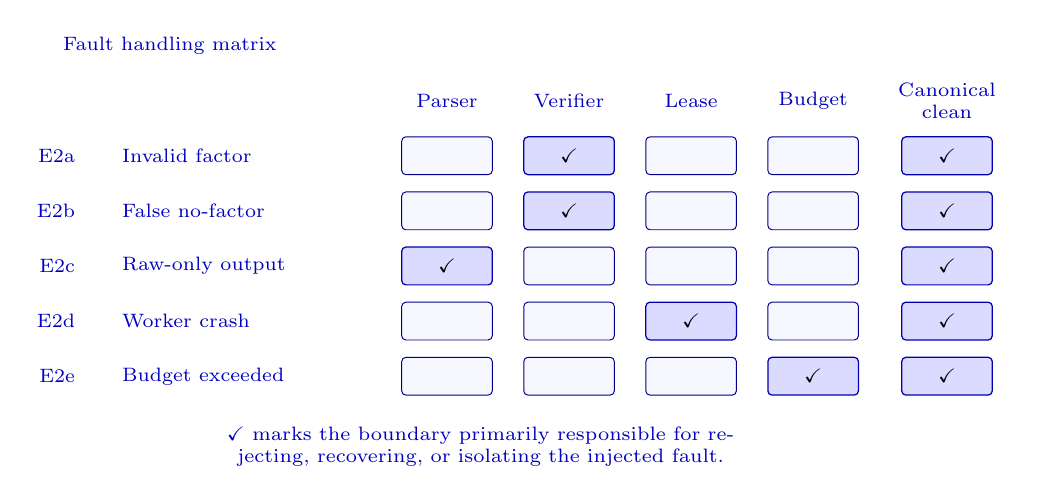
\begin{tikzpicture}[
  font=\scriptsize,
  rowlabel/.style={
    text=blue!75!black,
    anchor=east
  },
  faultlabel/.style={
    text=blue!75!black,
    anchor=west
  },
  header/.style={
    text=blue!75!black,
    align=center
  },
  cell/.style={
    draw=blue!55!black,
    fill=blue!3,
    rounded corners=1.5pt,
    line width=0.35pt,
    minimum width=1.15cm,
    minimum height=0.48cm,
    align=center
  },
  hitcell/.style={
    draw=blue!70!black,
    fill=blue!14,
    rounded corners=1.5pt,
    line width=0.45pt,
    minimum width=1.15cm,
    minimum height=0.48cm,
    align=center
  }
]

% Title
\node[
  font=\scriptsize,
  text=blue!75!black,
  anchor=west
] at (-5.4,3.55)
{Fault handling matrix};

% Column headers
\node[header] at (-0.4,2.85) {Parser};
\node[header] at (1.15,2.85) {Verifier};
\node[header] at (2.70,2.85) {Lease};
\node[header] at (4.25,2.85) {Budget};
\node[header, text width=1.65cm] at (5.95,2.85) {Canonical\\clean};

% ---------------- Row E2a ----------------
\node[rowlabel] at (-5.0,2.15) {E2a};
\node[faultlabel] at (-4.65,2.15) {Invalid factor};

\node[cell] at (-0.4,2.15) {};
\node[hitcell] at (1.15,2.15) {\(\checkmark\)};
\node[cell] at (2.70,2.15) {};
\node[cell] at (4.25,2.15) {};
\node[hitcell] at (5.95,2.15) {\(\checkmark\)};

% ---------------- Row E2b ----------------
\node[rowlabel] at (-5.0,1.45) {E2b};
\node[faultlabel] at (-4.65,1.45) {False no-factor};

\node[cell] at (-0.4,1.45) {};
\node[hitcell] at (1.15,1.45) {\(\checkmark\)};
\node[cell] at (2.70,1.45) {};
\node[cell] at (4.25,1.45) {};
\node[hitcell] at (5.95,1.45) {\(\checkmark\)};

% ---------------- Row E2c ----------------
\node[rowlabel] at (-5.0,0.75) {E2c};
\node[faultlabel] at (-4.65,0.75) {Raw-only output};

\node[hitcell] at (-0.4,0.75) {\(\checkmark\)};
\node[cell] at (1.15,0.75) {};
\node[cell] at (2.70,0.75) {};
\node[cell] at (4.25,0.75) {};
\node[hitcell] at (5.95,0.75) {\(\checkmark\)};

% ---------------- Row E2d ----------------
\node[rowlabel] at (-5.0,0.05) {E2d};
\node[faultlabel] at (-4.65,0.05) {Worker crash};

\node[cell] at (-0.4,0.05) {};
\node[cell] at (1.15,0.05) {};
\node[hitcell] at (2.70,0.05) {\(\checkmark\)};
\node[cell] at (4.25,0.05) {};
\node[hitcell] at (5.95,0.05) {\(\checkmark\)};

% ---------------- Row E2e ----------------
\node[rowlabel] at (-5.0,-0.65) {E2e};
\node[faultlabel] at (-4.65,-0.65) {Budget exceeded};

\node[cell] at (-0.4,-0.65) {};
\node[cell] at (1.15,-0.65) {};
\node[cell] at (2.70,-0.65) {};
\node[hitcell] at (4.25,-0.65) {\(\checkmark\)};
\node[hitcell] at (5.95,-0.65) {\(\checkmark\)};

% Bottom note
\node[
  font=\scriptsize,
  text=blue!75!black,
  align=center,
  text width=10.8cm
] at (0,-1.55)
{\(\checkmark\) marks the boundary primarily responsible for rejecting,
recovering, or isolating the injected fault.};

\end{tikzpicture}
}
}
\caption{\textcolor{blue}{Failure-handling matrix for Experiment~2. Each injected failure is handled by the relevant protocol boundary, and every case preserves zero canonical pollution.}}
\label{fig:failure-handling-matrix}
\end{figure}

These results show that executor submission is not equivalent to protocol
acceptance. A candidate output must pass the parser, verifier, and
canonical-selection boundary before it can affect accepted state. Invalid
evidence may remain auditable, but it does not become canonical evidence.

\FloatBarrier

\subsection{Experiment 3: Mechanism Ablation}
\label{subsec:exp3-ablation}

Experiment~3 disables one protection mechanism per run. The expected outcome is
not ordinary completion but controlled degradation. All five ablations are
reported as inconclusive, with completion rate 0.0 and no settlement. The
verifier ablation additionally produces one canonical pollution event, showing
the direct risk of bypassing plugin verification.

\begin{figure}[!htbp]
\centering
{\color{blue}
\begin{tikzpicture}[x=1.05cm,y=0.72cm]
  \node[tslabel, anchor=west] at (0,6.1) {Ablation outcome heatmap};

  \node[tssmall] at (4.1,5.35) {Completion};
  \node[tssmall] at (5.9,5.35) {Settlement};
  \node[tssmall] at (7.6,5.35) {Pollution};
  \node[tssmall] at (9.4,5.35) {Risk signal};

  \foreach \row/\case/\removed/\comp/\settle/\poll/\risk in {
    4.6/E3a/Verifier/0/0/1/Canonical,
    3.8/E3b/Parser policy/0/0/0/Raw boundary,
    3.0/E3c/Requeue/0/0/0/Stuck work,
    2.2/E3d/Merge gate/0/0/0/Premature merge,
    1.4/E3e/Slot check/0/0/0/Wrong slot
  }{
    \node[tslabel, anchor=east] at (1.1,\row) {\case};
    \node[tssmall, anchor=west] at (1.25,\row) {\removed};

    \node[tsbox, minimum width=0.7cm, minimum height=0.40cm] at (4.1,\row) {0.0};
    \node[tsbox, minimum width=0.7cm, minimum height=0.40cm] at (5.9,\row) {no};

    \ifnum\poll=1
      \node[tsdarkbox, minimum width=0.7cm, minimum height=0.40cm] at (7.6,\row) {1};
    \else
      \node[tsbox, minimum width=0.7cm, minimum height=0.40cm] at (7.6,\row) {0};
    \fi

    \node[tsbox, minimum width=2.45cm, minimum height=0.40cm] at (9.4,\row) {\risk};
  }

  \node[tssmall, anchor=west] at (0.8,0.45)
  {All ablations are inconclusive by design; E3a directly shows canonical pollution when verification is removed.};
\end{tikzpicture}
}
\caption{\textcolor{blue}{Mechanism-ablation heatmap. Removing core protections prevents normal completion; removing verification additionally creates canonical pollution.}}
\label{fig:ablation-heatmap}
\end{figure}

The ablation suite supports a mechanism-level claim: correctness is not a
property of the task solver alone, but of the solver together with parser
ownership, verification, lease recovery, merge gating, and slot integrity.

\FloatBarrier

\subsection{Experiment 4: Cross-Plugin Generality}
\label{subsec:exp4-cross-plugin}

Experiment~4 tests whether the protocol core can coordinate plugins with
different semantics. The factorization case and both Lean proof cases pass. The
Lean cases include real checker evidence, and the decomposition/merge case tests
a split-and-merge proof path rather than only a direct proof.

\begin{figure}[!htbp]
\centering
{\color{blue}
\resizebox{0.92\linewidth}{!}{%
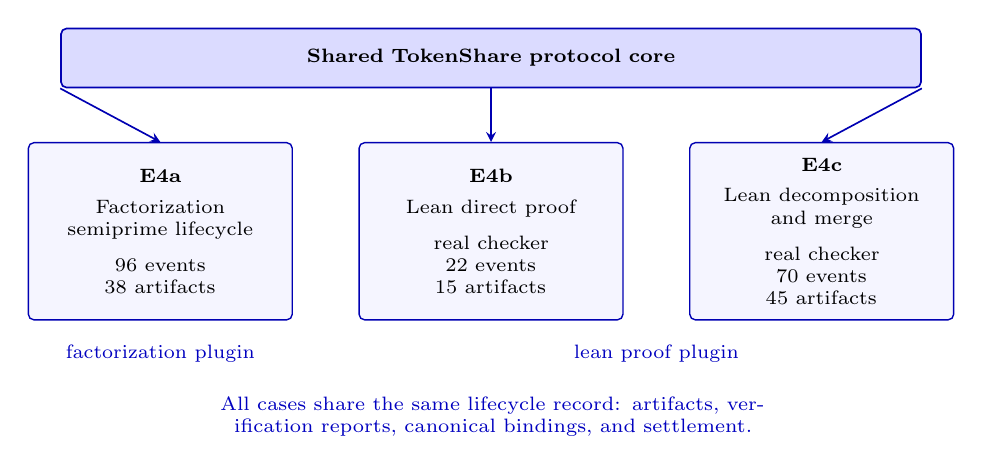
\begin{tikzpicture}[
  font=\scriptsize,
  box/.style={
    draw=blue!70!black,
    fill=blue!4,
    rounded corners=2pt,
    line width=0.5pt,
    align=center,
    inner sep=5pt
  },
  corebox/.style={
    draw=blue!70!black,
    fill=blue!14,
    rounded corners=2pt,
    line width=0.6pt,
    align=center,
    inner sep=6pt
  },
  arrow/.style={
    draw=blue!70!black,
    -stealth,
    line width=0.6pt
  }
]

% Top core box
\node[corebox, text width=10.5cm, minimum height=0.75cm] (core) at (0,3.2)
{\textbf{Shared TokenShare protocol core}};

% Three case cards
\node[box, text width=3.0cm, minimum height=2.25cm] (e4a) at (-4.2,1.0)
{\textbf{E4a}\\[3pt]
Factorization\\
semiprime lifecycle\\[5pt]
96 events\\
38 artifacts};

\node[box, text width=3.0cm, minimum height=2.25cm] (e4b) at (0,1.0)
{\textbf{E4b}\\[3pt]
Lean direct proof\\[5pt]
real checker\\
22 events\\
15 artifacts};

\node[box, text width=3.0cm, minimum height=2.25cm] (e4c) at (4.2,1.0)
{\textbf{E4c}\\[3pt]
Lean decomposition\\
and merge\\[5pt]
real checker\\
70 events\\
45 artifacts};

% Plugin labels
\node[font=\scriptsize, text=blue!75!black] at (-4.2,-0.55)
{factorization plugin};

\node[font=\scriptsize, text=blue!75!black] at (2.1,-0.55)
{lean proof plugin};

% Arrows from core to cases
\draw[arrow] (core.south west) -- (e4a.north);
\draw[arrow] (core.south) -- (e4b.north);
\draw[arrow] (core.south east) -- (e4c.north);

% Bottom note
\node[
  font=\scriptsize,
  text=blue!75!black,
  align=center,
  text width=10.5cm
] at (0,-1.35)
{All cases share the same lifecycle record: artifacts, verification reports,
canonical bindings, and settlement.};

\end{tikzpicture}
}
}
\caption{\textcolor{blue}{Cross-plugin generality in Experiment~4. The same protocol core supports both factorization and Lean proof plugins while domain semantics remain plugin-owned.}}
\label{fig:cross-plugin-map}
\end{figure}

\begin{table}[!htbp]
\centering
\caption{\textcolor{blue}{Experiment 4: cross-plugin generality results.}}
\label{tab:cross-plugin-results}
\footnotesize
{\color{blue}
\begin{tabularx}{0.96\linewidth}{
  @{}
  >{\raggedright\arraybackslash}p{0.10\linewidth}
  >{\raggedright\arraybackslash}p{0.24\linewidth}
  >{\raggedright\arraybackslash}p{0.22\linewidth}
  >{\raggedright\arraybackslash}X
  @{}
}
\toprule
Case & Workload and plugin & Evidence footprint & Interpretation \\
\midrule

E4a
&
\begin{minipage}[t]{\linewidth}
\textbf{Semiprime lifecycle}

Plugin: factorization
\end{minipage}
&
\begin{minipage}[t]{\linewidth}
Checker evidence: no

Events: 96

Artifacts: 38
\end{minipage}
&
\begin{minipage}[t]{\linewidth}
The arithmetic-search plugin completes the shared TokenShare lifecycle through plugin-owned factorization semantics.
\end{minipage}
\\[1.0em]

E4b
&
\begin{minipage}[t]{\linewidth}
\textbf{Lean direct proof}

Plugin: lean proof
\end{minipage}
&
\begin{minipage}[t]{\linewidth}
Checker evidence: yes

Events: 22

Artifacts: 15
\end{minipage}
&
\begin{minipage}[t]{\linewidth}
The direct proof path is accepted by a real Lean checker, showing that protocol acceptance can rely on external formal verification evidence.
\end{minipage}
\\[1.0em]

E4c
&
\begin{minipage}[t]{\linewidth}
\textbf{Lean decomposition and merge}

Plugin: lean proof
\end{minipage}
&
\begin{minipage}[t]{\linewidth}
Checker evidence: yes

Events: 70

Artifacts: 45
\end{minipage}
&
\begin{minipage}[t]{\linewidth}
The split child proofs and the merged root proof are accepted by the checker, demonstrating that the protocol can coordinate decomposition and merge beyond direct proof submission.
\end{minipage}
\\

\bottomrule
\end{tabularx}
}
\end{table}
The result supports the protocol generality claim. The core records lifecycle
state, artifacts, verification reports, canonical bindings, and settlement
records, while factorization arithmetic and Lean proof checking remain outside
the protocol core.

\FloatBarrier

\subsection{Auxiliary Simulation: Heterogeneous Contributors}
\label{subsec:aux-heterogeneous-contributors}

Because \TS{} targets shared token economies, we include a contributor-
heterogeneity simulation. This simulation is not a fifth experiment. It
approximates a multi-user setting by running the same semiprime task under three
executor profiles: a deterministic local contributor, a real model-backed
contributor, and a malformed raw-output contributor. The workload is
\(N=91\), with expected factors \([7,13]\).

The simulation tests the executor boundary. A model-backed contributor may
produce raw outputs, but the protocol does not directly trust those outputs. Raw
responses must be stored, parsed into the factorization output contract, and
verified before they can become useful evidence. The malformed profile models an
unreliable contributor: its output is preserved as evidence, but it produces a
parse-failure artifact rather than an accepted parsed result.

\begin{figure}[!htbp]
\centering
{\color{blue}
\resizebox{0.92\linewidth}{!}{%
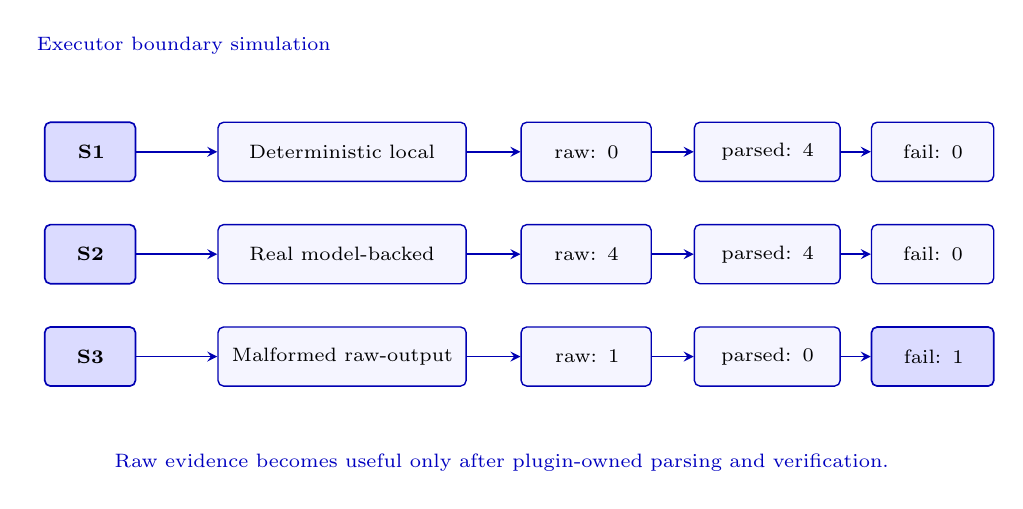
\begin{tikzpicture}[
  font=\scriptsize,
  box/.style={
    draw=blue!70!black,
    fill=blue!4,
    rounded corners=2pt,
    line width=0.5pt,
    align=center,
    inner sep=5pt
  },
  darkbox/.style={
    draw=blue!70!black,
    fill=blue!14,
    rounded corners=2pt,
    line width=0.6pt,
    align=center,
    inner sep=5pt
  },
  arrow/.style={
    draw=blue!70!black,
    -stealth,
    line width=0.6pt
  }
]

% Title
\node[font=\scriptsize, text=blue!75!black, anchor=west] at (-5.4,3.25)
{Executor boundary simulation};

% Row 1
\node[darkbox, text width=0.8cm, minimum height=0.75cm] (s1id) at (-4.6,1.9)
{\textbf{S1}};

\node[box, text width=2.8cm, minimum height=0.75cm] (s1type) at (-1.4,1.9)
{Deterministic local};

\node[box, text width=1.3cm, minimum height=0.75cm] (s1raw) at (1.7,1.9)
{raw: 0};

\node[box, text width=1.5cm, minimum height=0.75cm] (s1parsed) at (4.0,1.9)
{parsed: 4};

\node[box, text width=1.2cm, minimum height=0.75cm] (s1fail) at (6.1,1.9)
{fail: 0};

% Row 2
\node[darkbox, text width=0.8cm, minimum height=0.75cm] (s2id) at (-4.6,0.6)
{\textbf{S2}};

\node[box, text width=2.8cm, minimum height=0.75cm] (s2type) at (-1.4,0.6)
{Real model-backed};

\node[box, text width=1.3cm, minimum height=0.75cm] (s2raw) at (1.7,0.6)
{raw: 4};

\node[box, text width=1.5cm, minimum height=0.75cm] (s2parsed) at (4.0,0.6)
{parsed: 4};

\node[box, text width=1.2cm, minimum height=0.75cm] (s2fail) at (6.1,0.6)
{fail: 0};

% Row 3
\node[darkbox, text width=0.8cm, minimum height=0.75cm] (s3id) at (-4.6,-0.7)
{\textbf{S3}};

\node[box, text width=2.8cm, minimum height=0.75cm] (s3type) at (-1.4,-0.7)
{Malformed raw-output};

\node[box, text width=1.3cm, minimum height=0.75cm] (s3raw) at (1.7,-0.7)
{raw: 1};

\node[box, text width=1.5cm, minimum height=0.75cm] (s3parsed) at (4.0,-0.7)
{parsed: 0};

\node[darkbox, text width=1.2cm, minimum height=0.75cm] (s3fail) at (6.1,-0.7)
{fail: 1};

% Arrows row 1
\draw[arrow] (s1id.east) -- (s1type.west);
\draw[arrow] (s1type.east) -- (s1raw.west);
\draw[arrow] (s1raw.east) -- (s1parsed.west);
\draw[arrow] (s1parsed.east) -- (s1fail.west);

% Arrows row 2
\draw[arrow] (s2id.east) -- (s2type.west);
\draw[arrow] (s2type.east) -- (s2raw.west);
\draw[arrow] (s2raw.east) -- (s2parsed.west);
\draw[arrow] (s2parsed.east) -- (s2fail.west);

% Arrows row 3
\draw[arrow] (s3id.east) -- (s3type.west);
\draw[arrow] (s3type.east) -- (s3raw.west);
\draw[arrow] (s3raw.east) -- (s3parsed.west);
\draw[arrow] (s3parsed.east) -- (s3fail.west);

% Bottom note
\node[
  font=\scriptsize,
  text=blue!75!black,
  align=center,
  text width=10.4cm
] at (0.6,-2.05)
{Raw evidence becomes useful only after plugin-owned parsing and verification.};

\end{tikzpicture}
}
}
\caption{\textcolor{blue}{Executor-boundary outcomes in the contributor-heterogeneity simulation. The malformed contributor is recorded but not accepted.}}
\label{fig:executor-boundary-simulation}
\end{figure}

\begin{figure}[!htbp]
\centering
{\color{blue}
\resizebox{0.92\linewidth}{!}{%
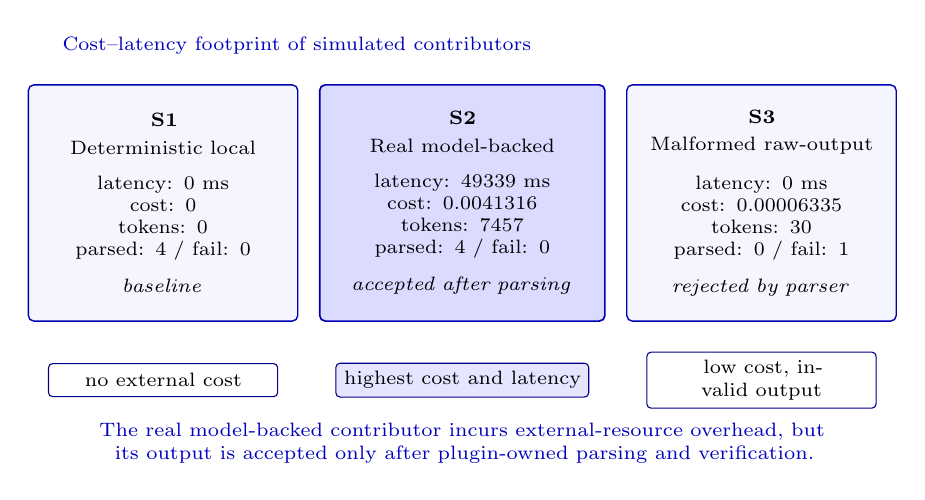
\begin{tikzpicture}[
  font=\scriptsize,
  card/.style={
    draw=blue!70!black,
    fill=blue!4,
    rounded corners=2pt,
    line width=0.5pt,
    align=center,
    inner sep=6pt
  },
  darkcard/.style={
    draw=blue!70!black,
    fill=blue!14,
    rounded corners=2pt,
    line width=0.6pt,
    align=center,
    inner sep=6pt
  },
  metric/.style={
    draw=blue!55!black,
    fill=white,
    rounded corners=1.5pt,
    line width=0.4pt,
    align=center,
    inner sep=3pt
  }
]

% Title
\node[
  font=\scriptsize,
  text=blue!75!black,
  anchor=west
] at (-5.2,3.0)
{Cost--latency footprint of simulated contributors};

% -------------------------------------------------------------------
% S1 card
% -------------------------------------------------------------------
\node[card, text width=3.0cm, minimum height=3.0cm] (s1) at (-3.8,1.0)
{
  \textbf{S1}\\[2pt]
  Deterministic local\\[6pt]

  \begin{tabular}{c}
  latency: 0 ms\\
  cost: 0\\
  tokens: 0\\
  parsed: 4 / fail: 0
  \end{tabular}\\[5pt]

  \textit{baseline}
};

% -------------------------------------------------------------------
% S2 card
% -------------------------------------------------------------------
\node[darkcard, text width=3.2cm, minimum height=3.0cm] (s2) at (0,1.0)
{
  \textbf{S2}\\[2pt]
  Real model-backed\\[6pt]

  \begin{tabular}{c}
  latency: 49339 ms\\
  cost: 0.0041316\\
  tokens: 7457\\
  parsed: 4 / fail: 0
  \end{tabular}\\[5pt]

  \textit{accepted after parsing}
};

% -------------------------------------------------------------------
% S3 card
% -------------------------------------------------------------------
\node[card, text width=3.0cm, minimum height=3.0cm] (s3) at (3.8,1.0)
{
  \textbf{S3}\\[2pt]
  Malformed raw-output\\[6pt]

  \begin{tabular}{c}
  latency: 0 ms\\
  cost: 0.00006335\\
  tokens: 30\\
  parsed: 0 / fail: 1
  \end{tabular}\\[5pt]

  \textit{rejected by parser}
};

% Visual comparison strip
\node[
  metric,
  text width=2.7cm,
  minimum height=0.42cm
] at (-3.8,-1.25)
{no external cost};

\node[
  metric,
  fill=blue!10,
  text width=3.0cm,
  minimum height=0.42cm
] at (0,-1.25)
{highest cost and latency};

\node[
  metric,
  text width=2.7cm,
  minimum height=0.42cm
] at (3.8,-1.25)
{low cost, invalid output};

% Bottom explanation
\node[
  font=\scriptsize,
  text=blue!75!black,
  align=center,
  text width=10.6cm
] at (0,-2.05)
{The real model-backed contributor incurs external-resource overhead,
but its output is accepted only after plugin-owned parsing and verification.};

\end{tikzpicture}
}
}
\caption{\textcolor{blue}{Cost--latency footprint of simulated contributor profiles. The model-backed contributor increases cost and latency, while the malformed contributor remains cheap but produces no accepted parsed output.}}
\label{fig:cost-latency-footprint}
\end{figure}

The deterministic and real model-backed profiles have identical correctness and
parser success:
\[
  \Delta_{\mathrm{correctness}}=0,\qquad
  \Delta_{\mathrm{parser}}=0.0,\qquad
  \Delta_{\mathrm{retry}}=0.
\]
The real model-backed path introduces external-resource overhead:
\[
  \Delta_{\mathrm{cost}}=0.0041316,\qquad
  \Delta_{\mathrm{latency}}=49339\ \mathrm{ms}.
\]
This simulation supports the shared-token interpretation of the protocol:
contributors may differ in execution medium, reliability, and cost, but their
outputs are mediated by a common parser, verifier, artifact, and accounting
interface.

\FloatBarrier

\subsection{Audit Footprint}
\label{subsec:audit-footprint}

The default suite records 1215 events and 510 artifacts. This footprint is not
only execution telemetry; it is the protocol evidence used for replay, audit,
canonical-state inspection, and contribution accounting.

\begin{figure}[!htbp]
\centering
{\color{blue}
\begin{tikzpicture}[x=0.0085cm,y=0.0042cm]
  \node[tslabel, anchor=west] at (0,1330) {Cumulative audit footprint};

  % axes
  \draw[tsline] (0,0) -- (1300,0);
  \draw[tsline] (0,0) -- (0,1250);

  \foreach \y/\lab in {0/0,400/400,800/800,1200/1200} {
    \draw[blue!15] (0,\y) -- (1250,\y);
    \node[tssmall, anchor=east] at (-30,\y) {\lab};
  }

  \foreach \x/\lab in {300/Exp.1,600/Exp.2,900/Exp.3,1200/Exp.4} {
    \draw[tsline] (\x,15) -- (\x,-15);
    \node[tssmall, anchor=north] at (\x,-40) {\lab};
  }

  % cumulative events
  \draw[blue!70!black, line width=0.9pt]
    (300,362) -- (600,842) -- (900,1027) -- (1200,1215);
  \foreach \x/\y in {300/362,600/842,900/1027,1200/1215}{
    \filldraw[draw=blue!70!black, fill=blue!35] (\x,\y) circle (3pt);
  }

  % cumulative artifacts
  \draw[blue!40!black, line width=0.9pt, dashed]
    (300,147) -- (600,337) -- (900,412) -- (1200,510);
  \foreach \x/\y in {300/147,600/337,900/412,1200/510}{
    \filldraw[draw=blue!40!black, fill=blue!8] (\x,\y) rectangle +(6,6);
  }

  \node[tssmall, anchor=west] at (850,1110) {cumulative events};
  \node[tssmall, anchor=west] at (850,455) {cumulative artifacts};
\end{tikzpicture}
}
\caption{\textcolor{blue}{Cumulative audit footprint across Experiments~1--4. The monotone increase reflects accumulated replay and artifact evidence, not merely final-answer records.}}
\label{fig:cumulative-audit-footprint}
\end{figure}

\begin{table}[!htbp]
\centering
\caption{\textcolor{blue}{Event and artifact footprint by experiment group.}}
\label{tab:audit-footprint}
\small
{\color{blue}
\begin{tabularx}{0.86\linewidth}{X>{\centering\arraybackslash}p{0.11\linewidth}>{\centering\arraybackslash}p{0.11\linewidth}>{\centering\arraybackslash}p{0.13\linewidth}>{\centering\arraybackslash}p{0.13\linewidth}}
\toprule
Group & Runs & Passed & Events & Artifacts \\
\midrule
Experiment 1 & 4 & 4 & 362 & 147 \\
Experiment 2 & 5 & 5 & 480 & 190 \\
Experiment 3 & 5 & 0 & 185 & 75 \\
Experiment 4 & 3 & 3 & 188 & 98 \\
\midrule
Total & 17 & 12 & 1215 & 510 \\
\bottomrule
\end{tabularx}
}
\end{table}

\FloatBarrier

\subsection{Limitations}
\label{subsec:limitations}

The results provide prototype-scale protocol evidence rather than a large-scale
performance benchmark. The factorization tasks are fixed small integers, the
default deterministic suite uses one seed, and the contributor-heterogeneity
simulation uses a small number of executor profiles rather than a large
population of real users. Accordingly, the evidence supports lifecycle
completeness, canonical-state safety, mechanism necessity, cross-plugin
execution, and AI-output auditability. Throughput scaling, stronger adversarial
workloads, and multi-provider cost optimization remain separate evaluation
targets.

\subsection{Summary}
\label{subsec:experiment-summary}

The experiments support four main conclusions. First, the factorization plugin
completes end-to-end lifecycle cases with correct outputs and settlement.
Second, injected failures do not pollute canonical state. Third, disabling key
mechanisms produces the expected degradation. Fourth, the same protocol core
supports factorization and real Lean proof plugins. The auxiliary contributor
simulation further shows how heterogeneous users or executors can be mediated by
the same raw-output, parser, verifier, artifact, and accounting boundary.

% Restore the original caption behavior and text color after this section.
\makeatletter
\let\@makecaption\TSoldmakecaption
\makeatother
\endgroup
\normalcolor



\section{How to Join TokenShare}


% decompose + merge
% regester 



\section{Related Work}

\paragraph{Distributed task allocation and market coordination.}
TokenShare builds on a long line of work on allocating work among distributed agents. The Contract Net Protocol introduced a negotiation pattern in which tasks are announced, potential contractors bid, and managers award work to selected agents \citep{smith1980contract}. Multi-robot task allocation later formalized the relation among agents, tasks, utilities, costs, and assignment structure \citep{gerkey2004formal}, while market-based coordination studied how decentralized bidding mechanisms can trade off communication cost, robustness, and solution quality \citep{dias2006market}. These works justify treating contributor selection as a protocol-level allocation problem. TokenShare differs in that the allocated object is not a single atomic job: it is a recursively expandable task tree or DAG whose leaves may require model tokens, tools, local computation, or human judgment, and whose rewards are delayed until verification and merge succeed.

\paragraph{Complex crowdsourcing and decentralized crowdsourcing.}
Human-computation systems show that complex work can be decomposed, distributed, reviewed, and recomposed. CrowdForge proposes partition, map, and reduce primitives for crowdsourcing complex work \citep{kittur2011crowdforge}, and Turkomatic explores recursive task and workflow design for Mechanical Turk-style settings \citep{kulkarni2011turkomatic}. Blockchain-based crowdsourcing systems such as CrowdBC and decentralized HIT protocols add payments, dispute handling, and reduced reliance on centralized platforms \citep{li2018crowdbc,liang2022decentralizedhit}. These systems are important precedents for TokenShare's task publication, contribution accounting, and settlement layer. Their main limitation for our setting is that they are usually designed around human microtasks or fixed crowdsourcing workflows, whereas TokenShare targets heterogeneous intelligent work involving LLM agents, local tools, verifiers, recursive decomposition, and task-specific acceptance functions.

\paragraph{Volunteer and distributed execution systems.}
Volunteer and cluster-computing systems provide practical lessons for unreliable and heterogeneous execution. BOINC supports volunteer scientific computation over devices that differ in capability, availability, and reliability \citep{anderson2020boinc}. MapReduce popularized partitioned data processing with automatic scheduling, failure handling, and re-execution on commodity clusters \citep{dean2004mapreduce}. Ray supports dynamic task graphs for AI applications \citep{moritz2018ray}, while Sparrow studies decentralized low-latency scheduling for short parallel tasks \citep{ousterhout2013sparrow}. TokenShare borrows the engineering vocabulary of leases, checkpoints, heartbeats, redundant execution, and reassignment. Its focus, however, is semantic and verifiable intelligent production rather than only data-parallel computation: a work unit must include an input schema, output schema, verifier, provenance record, and merge rule.

\paragraph{Blockchains, verifiable computation, and useful work.}
Bitcoin demonstrates that mutually untrusted participants can be coordinated through a public ledger and proof-of-work incentives \citep{nakamoto2008bitcoin}. Ethereum generalizes the ledger into programmable smart contracts for decentralized applications \citep{buterin2014ethereum}. TrueBit studies interactive verification for off-chain computation, allowing expensive computations to be checked by blockchain-linked protocols \citep{teutsch2019truebit}. Proof-of-useful-work systems such as Ofelimos attempt to replace artificial hash puzzles with useful optimization work \citep{fitzi2022ofelimos}. TokenShare is adjacent to these systems but has a different objective: it is not a consensus protocol and does not require useful work to secure a blockchain. Instead, it uses ledgered commitments, verification records, and settlement rules to coordinate useful AI- and human-assisted production.

\paragraph{LLM decomposition, tool use, and multi-agent workflows.}
Recent LLM research shows that complex reasoning benefits from explicit intermediate structure. Decomposed Prompting, Least-to-Most Prompting, Tree of Thoughts, and ReAct all externalize decomposition, search, tool use, or intermediate reasoning states \citep{khot2023decomposed,zhou2023least,yao2023tree,yao2023react}. HuggingGPT and related tool-use systems use an LLM to plan subtasks and route them to external models or tools \citep{shen2023hugginggpt}. Multi-agent frameworks such as CAMEL, AutoGen, MetaGPT, and ChatDev further introduce role specialization, agent communication, and structured software-production workflows \citep{li2023camel,wu2023autogen,hong2024metagpt,qian2023chatdev}. These works motivate TokenShare's use of decomposition, roles, and tool-facing agents. The gap is that most LLM-agent systems assume a trusted orchestrator and evaluate final task success, while TokenShare treats resource allocation, failure recovery, verifier selection, contribution provenance, and reward settlement as first-class protocol objects.

\paragraph{Verification-heavy intelligent tasks.}
Formal proof assistants provide a useful testbed because accepted outputs can be checked deterministically. The Lean mathematical library shows how a large community can maintain formalized mathematics in Lean \citep{mathlib2020}. miniF2F provides a cross-system benchmark for formal olympiad-level mathematics \citep{zheng2021minif2f}, and LeanDojo exposes Lean proof states, premises, interaction data, and benchmarks for retrieval-augmented theorem proving \citep{yang2023leandojo}. These works support our Lean proof-production application: TokenShare can treat a theorem, subgoal, tactic patch, error log, or auxiliary lemma as a task unit, while Lean supplies a replayable verifier.

\paragraph{Annotation quality and low-resource public-good NLP.}
Crowdsourced annotation research provides mature models for noisy contributors and uncertain labels. Dawid--Skene style aggregation estimates latent labels and worker error rates \citep{dawid1979maximum}; GLAD models both annotator ability and item difficulty \citep{whitehill2009glad}; MACE estimates annotator competence under noisy or adversarial conditions \citep{hovy2013mace}; and Snorkel shows how weak supervision sources can be combined into probabilistic labels \citep{ratner2017snorkel}. Low-resource language work also warns that public-good NLP is not merely a data-scarcity problem: language technologies are unevenly distributed across the world's languages \citep{joshi2020state}, participatory projects such as Masakhane emphasize community involvement \citep{nekoto2020participatory}, and NLLB combines large-scale data construction with human-centered evaluation for many languages \citep{nllb2022}. These lines motivate TokenShare's emphasis on provenance, uncertainty, expert escalation, and community review rather than treating generated artifacts as automatically authoritative.





\begin{table}[t]
\centering
\small
\caption{Positioning of TokenShare relative to adjacent work.}
\label{tab:related_positioning}
\begin{tabularx}{\linewidth}{p{0.22\linewidth} X X}
\toprule
Line of work & Main contribution & Gap addressed by TokenShare \\
\midrule
Task allocation & Negotiated or market-based assignment among agents & Recursive task DAGs with verification-aware routing and delayed settlement \\
Complex crowdsourcing & Human workflow decomposition and recomposition & Heterogeneous LLM, tool, compute, and human contributors with typed verifiers \\
Distributed execution & Scheduling and recovery for unreliable machines & Semantic intelligent work units with provenance, audit, and merge rules \\
Blockchain and smart contracts & Trustless ledgers, programmable settlement, verifiable off-chain computation & Useful contribution accounting rather than artificial proof-of-work or consensus mining \\
LLM-agent systems & Planning, tool use, role specialization, and agent communication & Fault tolerance, resource sharing, contribution attribution, and protocol-level incentives \\
\bottomrule
\end{tabularx}
\end{table}


\section{Conclusion}

This paper proposes TokenShare, a protocol for turning idle tokens, local computation, tool-execution capacity, and human effort into useful distributed intelligent work. Instead of treating AI tasks as isolated prompt-response interactions, TokenShare frames large public-good tasks as recursively decomposable, verifiable, fault-tolerant, and ledger-recorded production processes.

The key idea is simple: large tasks can be divided into smaller units, assigned to heterogeneous contributors, locally and globally verified, recursively merged, and rewarded according to transparent protocol rules. By combining ideas from decentralized ledgers, smart contracts, crowdsourcing, distributed systems, and multi-agent AI, TokenShare aims to move from artificial proof-of-work toward useful proof-of-contribution.

The protocol is not intended to make all tasks distributed or decentralized. For small or weakly decomposable tasks, coordination overhead may outweigh the benefits. Its value is expected to appear in tasks that are large, modular, verification-heavy, and socially meaningful. Future work will implement TokenShare on concrete benchmarks such as low-resource language knowledge organization and multi-source annotation, and evaluate whether shared token economics can provide a reliable foundation for scalable public-good AI collaboration.


\section*{Ethical considerations}

The protocol is intended for public-good production, but public-good framing does not remove risk. Low-resource language work can expose community knowledge, cultural context, and identity. Early experiments will therefore use synthetic languages. Real-language studies require licensing review, community consent, careful data governance, and expert validation. Annotation tasks may include sensitive data; the protocol must support privacy constraints, minimal disclosure, and source-specific access control. The ledger should support accountability and reward attribution, but it must not become a coercive surveillance mechanism. Finally, model-generated content must preserve uncertainty flags and should never be presented as community-authoritative without appropriate human or community review.



\bibliographystyle{plainnat}
\bibliography{reference}

\section{Implementation Todo List}

\subsection{Phase 1: Shared TokenShare Harness}

\begin{itemize}[leftmargin=*]
  \item Implement task registry with root task creation, task ids, and task states.
  \item Implement task graph with parent-child dependencies and checkpoint status.
  \item Implement lease state transitions: \texttt{Pending}, \texttt{Leased}, \texttt{Submitted}, \texttt{Verified}, \texttt{Rejected}, \texttt{Expired}, \texttt{Merged}.
  \item Implement timeout detection and re-queue.
  \item Implement the common verifier interface.
  \item Implement ledger logging with structured JSON or CSV output.
  \item Implement synthetic client profiles: fast, slow, unreliable, invalid, offline, and high-reputation.
  \item Implement experiment configuration files for seeds, client count, failure rate, timeout, redundancy, and budget.
\end{itemize}

\subsection{Phase 2: Factorization Experiments}

\begin{itemize}[leftmargin=*]
  \item Generate factorization benchmark instances with hidden factors.
  \item Implement search-range decomposition.
  \item Implement factorization clients.
  \item Implement modular verification for factor candidates.
  \item Implement negative range certificates.
  \item Implement factorization baselines.
  \item Run pilot experiments on small integers.
  \item Run full experiments over bit length, client count, failure rate, lease duration, and checkpoint policy.
  \item Export aggregate metrics and raw logs.
\end{itemize}

\subsection{Phase 3: Lean Experiments}

\begin{itemize}[leftmargin=*]
  \item Freeze Lean, Mathlib, Lake, and environment hash.
  \item Select theorem benchmark sets.
  \item Build theorem-to-root-task conversion.
  \item Implement Lean verifier with canonical replay.
  \item Implement direct proof submissions.
  \item Implement decomposition submissions with subgoals and merge rules.
  \item Implement error-log repair tasks.
  \item Implement checkpoint reuse for verified subproofs.
  \item Implement Lean baselines.
  \item Run pilot experiments on small theorem sets.
  \item Run full experiments over theorem difficulty, token budget, client count, failure rate, and decomposition depth.
  \item Export aggregate metrics and raw logs.
\end{itemize}

\subsection{Phase 4: Analysis and Reporting}

\begin{itemize}[leftmargin=*]
  \item Plot client count versus completion time.
  \item Plot failure rate versus recovery time.
  \item Compare checkpoint and no-checkpoint conditions.
  \item Compare TokenShare against all baselines.
  \item Run audit replay from ledger logs.
  \item Identify negative cases where coordination overhead dominates.
  \item Prepare tables for success rate, cost, recovery, and auditability.
  \item Write the experimental results section using both aggregate metrics and failure analysis.
\end{itemize}

\section{Minimum Success Criteria}

The experimental phase is ready for paper reporting when:
\begin{itemize}[leftmargin=*]
  \item Each application has at least one successful end-to-end TokenShare run.
  \item Each baseline can be executed under the same benchmark configuration.
  \item Raw logs can reproduce aggregate metrics.
  \item Audit replay can reconstruct at least one successful final output from ledger records.
  \item Failure cases are preserved rather than discarded.
  \item The experiment scripts can be rerun from fixed configuration files and random seeds.
\end{itemize}

\end{document}
